% This file should be replaced with your file with thesis content.
%=========================================================================
% Authors: Michal Bidlo, Bohuslav Křena, Jaroslav Dytrych, Petr Veigend and Adam Herout 2019

% For compilation piecewise (see projekt.tex), it is necessary to uncomment it and change
% \documentclass[../projekt.tex]{subfiles}
% \begin{document}

\chapter{Introduction}

Information plays a key role in our lives and understanding the world which surrounds us. There is no doubt that information is the most valuable resource, so with the increasing power of our computers, our ways of obtaining information are developing incredibly fast. As a species, we strive to receive, analyze, and produce as much information as possible. About half a century ago, the Mariner 4 spacecraft approached Mars and for the first time in the history of mankind took several pictures of another planet. After the camera took a picture, the image was sent as a digital code to Earth. Then data had to be passed through a decoder after receiving. This operation took several hours to process a single image. NASA employees did not want to wait that long and decided to decode the image manually, drawing the received message by hand. Therefore, it turned out that the world's first image of Mars was not a photo, but a hand-colored drawing. Nowadays, in a matter of minutes, we receive high-quality images from Mars, which are taken by the Ingenuity Martian helicopter assembled from smartphone chips. Moreover, the majority of time is spent overcoming interplanetary distance rather than decompressing data. We are getting terabytes of data from on-Earth surveys, while space observations, constrained by download bandwidth, deliver gigabytes per hour.

If the example above doesn't look convincing enough, here are some numbers that \emph{Forbes} cites in its article \enquote{175 Zettabytes by 2025}. According to this article, it is projected that the amount of digital data generated by mankind will grow from 33 ZB in 2018 to 175 ZB by 2025. It means that the amount of information will increase fivefold in the last seven years. This leads to the main problem. Traditional data analysis methods are not keeping up with the growing amount of information. In recent years, the rapid advancement of Artificial Intelligence (AI) and Machine Learning (ML) has transformed various industries, leading to the development of innovative solutions for complex data analysis. AI has not only accelerated data processing but has also achieved remarkable results in areas where traditional methods face challenges. One such area is astronomy, where the massive volumes of data generated by modern astronomical surveys make manual analysis techniques ineffective.

The main goal of this thesis is not only to explore how AI can be applied to image classification but also to showcase the entire process of developing a modern AI-based application that utilizes machine learning for image classification tasks. We will investigate the integration of such an application with advanced cloud-based platforms like Red Hat OpenShift. That application serves as the resulting product, reflecting the knowledge and skills that will be gained while working on this thesis. This includes a fundamental knowledge of astronomy, galaxy morphology, and an understanding of Machine Learning and Vision Transformer architectures. The techniques for preparing and augmenting the dataset for model training will be explained. Sequentially, the issues related to the training of the AI model will be addressed. This thesis also covers the steps on how to make the training process faster. The final model will be used in the web application that will be deployed into a hybrid cloud solution such as Red Hat OpenShift Container Platform. 

The author believes that the experience, which has been gained while working on this thesis, can be a valuable basis for the future, more comprehensive applications. Additionally, it could serve as a useful guide for engineers who are just beginning their journey in the development of applications whose core functionality relies on artificial intelligence.

%=========================================================================

\chapter{Galaxy And Its Morphology}

This chapter provides an overview of galaxies and the differences between their types. This background information is important for understanding the purpose of the study and assessing the quality of the data that will be presented in later chapters. The chapter discusses the reasons for studying galaxy morphology and the various types of galaxies.

\section{Why Study Galaxies}

The reason to study galaxies is that galaxies are the key to understanding the evolution of our entire Universe. By looking at \autoref{fig:DeepFiled}, we see a huge variety of galaxies. Galaxies are the largest stellar systems, primarily responsible for star formation and element synthesis. They contain a majority of luminous matter: stars, stellar remnants, interstellar gas, and dust, together with dark matter. Galaxies trace large-scale structure in the Universe and cosmic history over 13 billion years \cite{Hickson2016ASTR505}. The history of the Universe has been completely acquired by studying the formation and evolution of galaxies.

\begin{figure}[htbp]
    \centering
    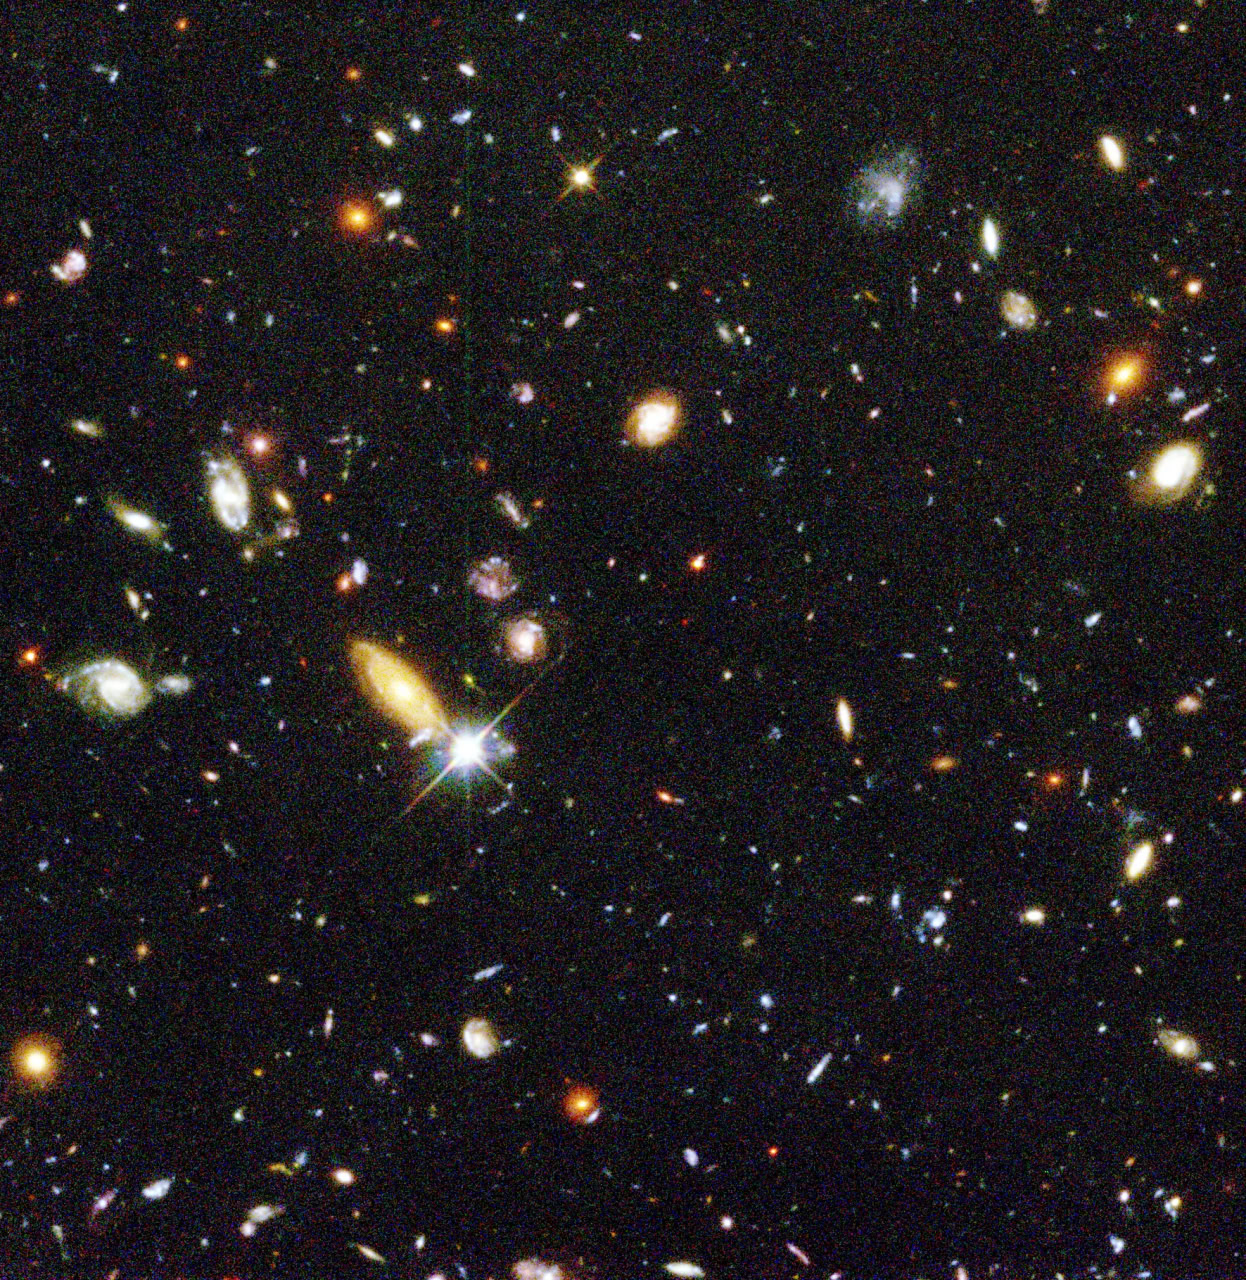
\includegraphics[width=0.45\textwidth]{obrazky-figures/02-theoretical-basis/deep-field.jpg}
    \caption{Hubble Deep Field (\url{https://science.nasa.gov/mission/hubble/science/universe-uncovered/hubble-deep-fields/}).}
    \label{fig:DeepFiled}
\end{figure}

Galaxies demonstrate a wide range of morphologies at different evolutionary stages. Early-type galaxies are always reddish in color. They contain the older stellar population and shell structures left by multiple galaxy mergers. These galaxies are mainly located in dense environments and appear elliptical in the view of morphology. Late-type galaxies have a bluish color and their star population is relatively young, containing ample cold gas and showing star formation activities in an intense way. Stars in late-type galaxies primarily exhibit rotational motion around the center, resulting in a disk-shaped galaxy with a stellar disk and spiral arms. Morphology and structure are particularly important, since they serve as a key for understanding how the galaxy’s physical parameters evolve over time \cite{van1998galaxy}.

\section{Galaxy Morphological Types}

Galaxies demonstrate a diverse range of morphological types. In this section, we will provide a brief overview of the primary classes of galaxies. The first to gain universal acceptance was proposed by Edwin Hubble, who arranged galaxies in his famous “Tuning Fork” diagram, demonstrated at \autoref{fig:fork}. The tuning fork scheme divides regular galaxies into four broad categories: ellipticals, lenticulars, spirals, and irregular shapes. The Hubble sequence is the most widely used system for categorizing galaxies, although there are variations of this system that have been expanded by different researchers \cite{Bonham2022Galaxies}.

\begin{figure}[htbp]
    \centering
    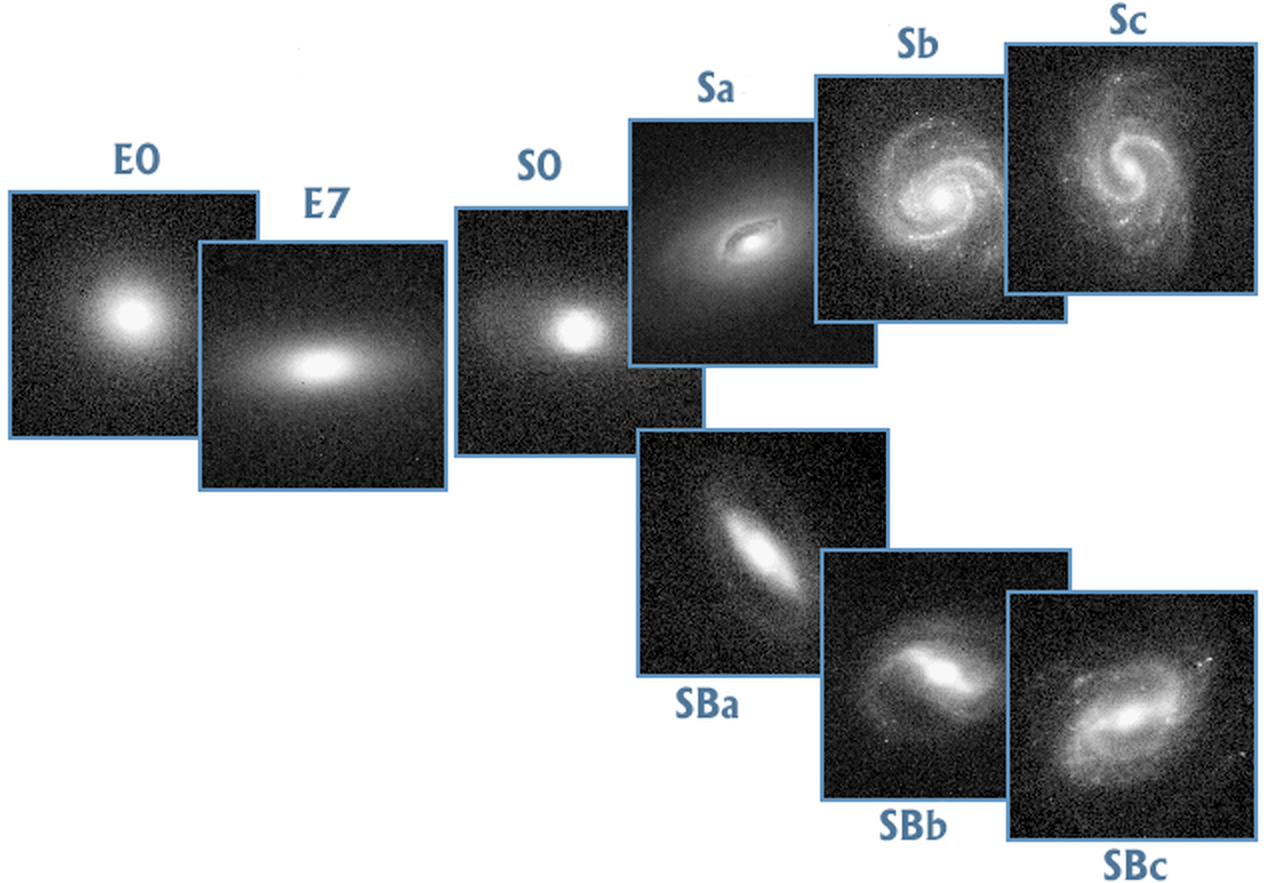
\includegraphics[width=0.6\textwidth]{obrazky-figures/02-theoretical-basis/tfork_upscaled.png}
    \caption{Hubble's Tunning Fork \cite{Hickson2016ASTR505}.}
    \label{fig:fork}
\end{figure}

\textbf{Spiral Galaxies}, as can be understood from the name, have a spiral pattern and visible component parts. This type of galaxy is characterized by the presence of a distinct disk with abundant gas, dust, and ongoing star formation. Spiral galaxies consist of 3 main components: Bulge is a large, spheroidal, tightly packed group of older stars. Many bulges are thought to host a supermassive black hole at their centers. Disk (spiral arms) is regions of stars that extend from the center of barred and unbarred spiral galaxies. They contain younger, bluer stars. Halo is an extended, roughly spherical component of a galaxy that extends beyond the main, visible component. It contains old clusters of stars (globular clusters).

\medskip

\textbf{Barred Galaxies} are a type of spiral galaxy that has bar-shaped elongations of stars throughout the center that “connect” two arms bent around. As the galaxy type progresses from Sa to Sc, the spiral arms increase in prominence and become less tightly wound and more irregular. The diffuse central bulge becomes less prominent.

\medskip

\textbf{Elliptical Galaxies} (denoted E) are characterized by a spheroidal shape and a symmetric, equal distribution of stars in all directions. There is little or no evidence of dust, gas, or star formation. New star formations are not present in elliptical galaxies. The star population in these galaxies is old. These galaxies have variation in ellipticity and position angle with radius (E0-E7).

\medskip

\textbf{Lenticular Galaxies} (denoted S0) are a type of galaxy intermediate between an elliptical and a spiral galaxy in galaxy morphological classification schemes. They are more flattened than elliptical galaxies and have a noticeable disk. The ring contains younger stars, which are very bright and blue-colored.

\medskip

\textbf{Irregular Galaxies} don’t have a particular pattern or symmetry in their shape, but they are very common in our universe. Irregular galaxies are often small in size and have younger, hotter stars.

\medskip

\textbf{Dwarf Galaxies} are small galaxies that contain several million to a billion stars and are the most common type of galaxy. They come in a wide variety of shapes and sizes.

\medskip

\textbf{Ring Galaxies} have the ring containing many massive, relatively young blue stars, which are extremely bright. The central region contains relatively little luminous matter. There are no spiral arms connecting the center with the ring.

\medskip

\textbf{Starburns Galaxies} are one undergoing an exceptionally high rate of star formation. The star formation of this type of galaxy is 100 times greater than we can see in the Milky Way galaxy.

\begin{figure}[htbp]
    \centering
    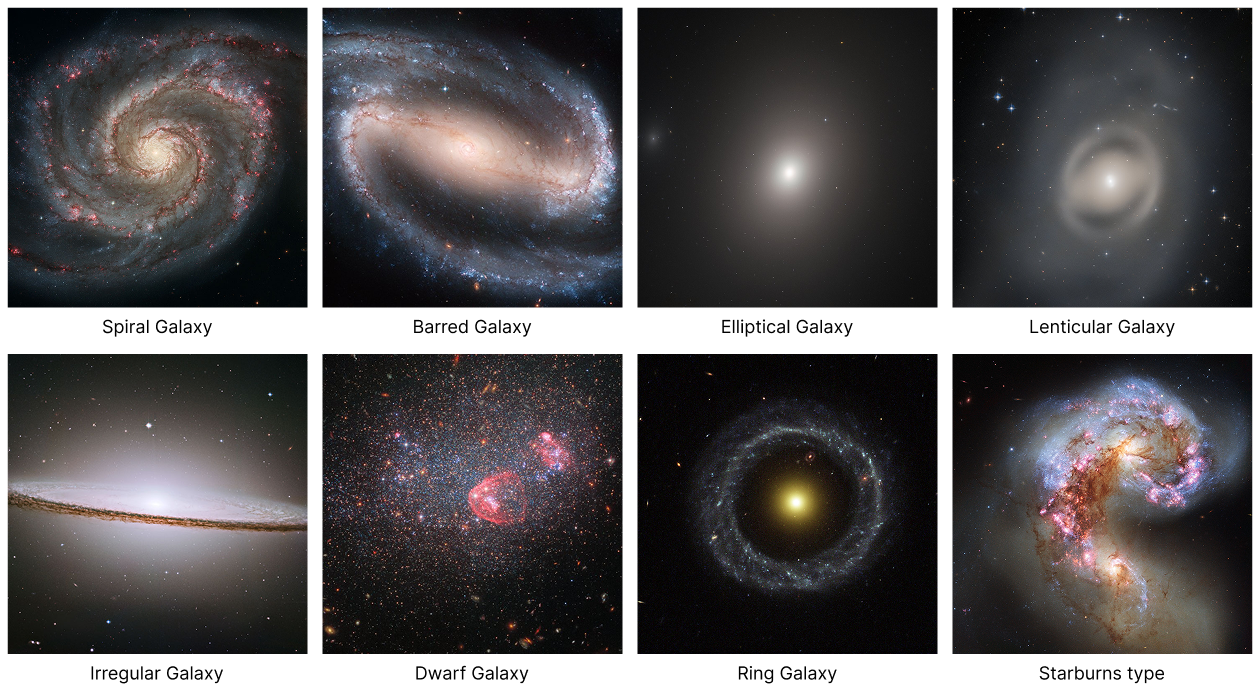
\includegraphics[width=\textwidth]{obrazky-figures/02-theoretical-basis/galaxies-types.png}
    \caption{Photos of Galaxies with Different Morphological Types (\url{https://esahubble.org/images/}).}
\end{figure}

\subsection*{Why Type of Galaxy Matter?}

The classification of galaxies is essential for understanding the variety of structures and evolutionary paths that galaxies can take. The shape and type provide important information about galaxies' properties, formation processes, and evolutionary paths. By analyzing how different types of galaxies are distributed across our universe, astronomers can understand the physical processes that shaped galaxies over billions of years. 

\begin{figure}[htbp]
    \centering
    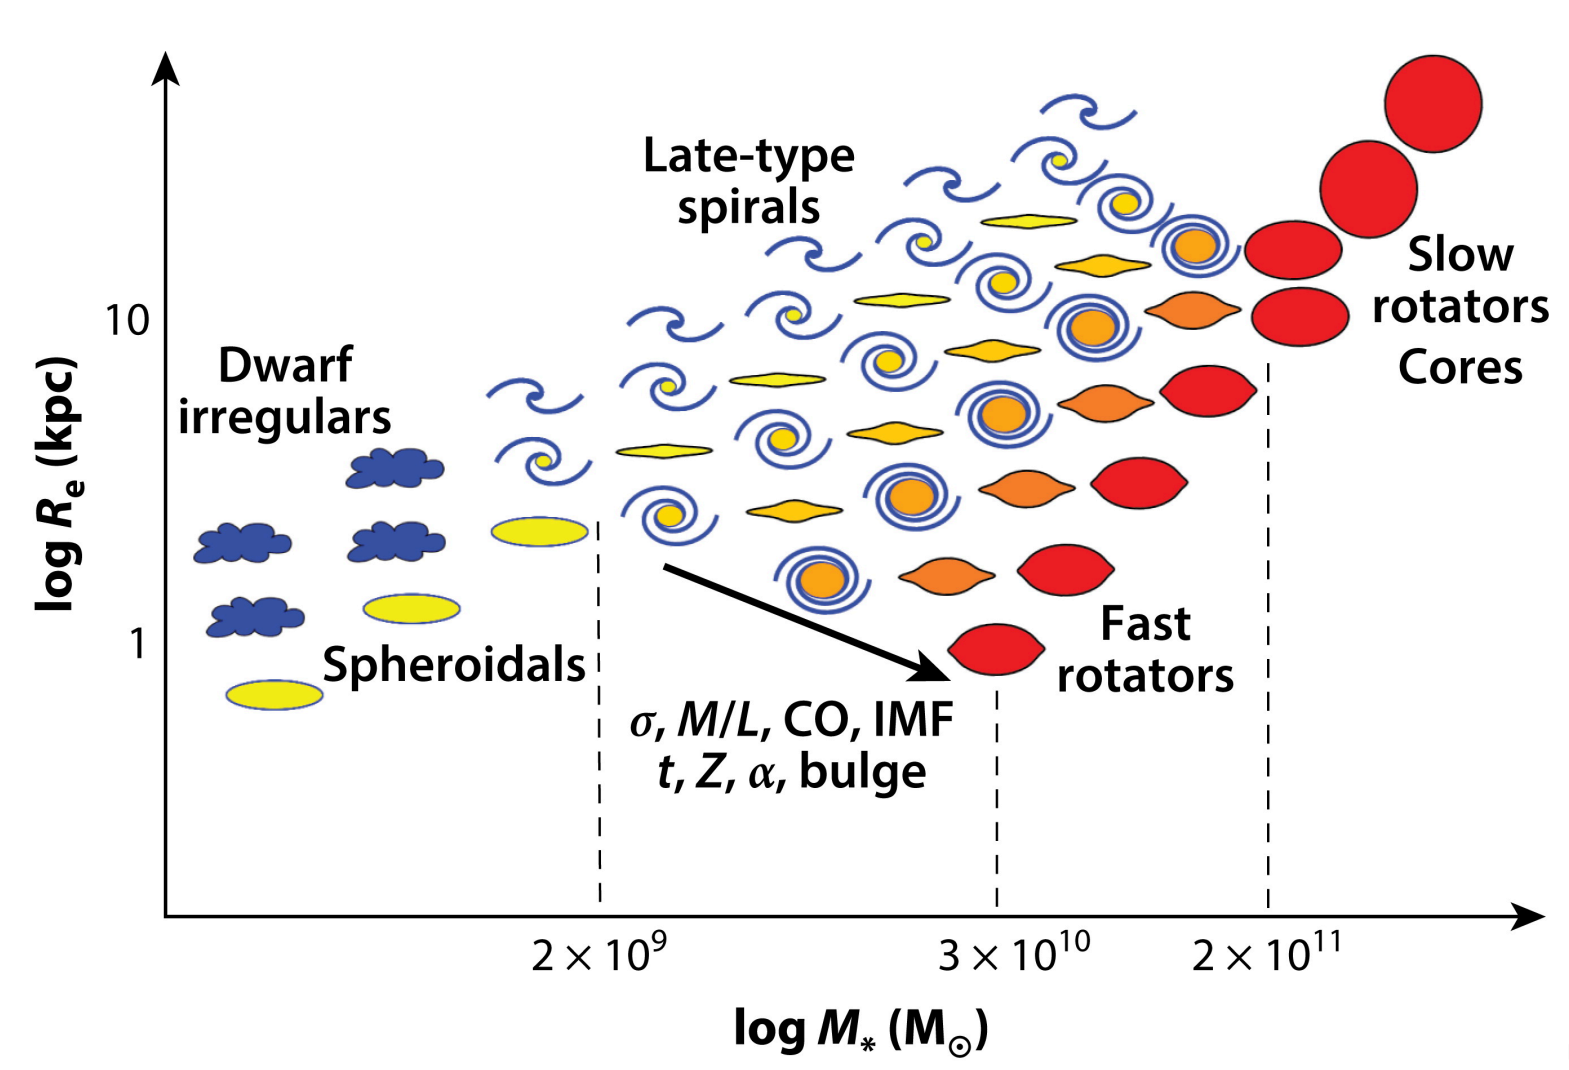
\includegraphics[width=0.6\textwidth]{obrazky-figures/02-theoretical-basis/types.png}
    \caption{Galaxy evolution on the mass-size diagram (\url{https://www.aip.de/media/thesis/sabine-thater-doktorarbeit.pdf}).}
    \label{fig:galaxy types}
\end{figure}

\autoref{fig:galaxy types} shows a correlation between galaxies' shapes and mass. Dwarf irregulars and spheroidals are in the low-mass region, late-type galaxies with intermediate masses, and early-type galaxies are divided into fast and slow rotators. The sequence of late-type galaxies aligns smoothly with the sequence of early-type galaxies. Massive galaxies are dominated by round or weakly triaxial slow rotators. Classifying galaxies according to their morphological characteristics is essential for effective data analysis \cite{cao2024galaxy}.

\section{Modern Galaxy Surveys and AI Applications}
\label{sec:modern-app}

Earlier sky surveys produced only modest amounts of data. For instance, the National Geographic Society-Palomar Observatory Sky Survey from 1958 collected just under 2,000 photographic plates of the night sky. Nowadays, the observations such as Sloan Digital Sky Survey (SDSS), James Webb Space Telescope (JWST) and other survey projects generate massive amounts of astronomical data. For example, only the SDSS survey has produced photometric observations of nearly one billion unique objects across five filters, covering roughly one-third of the sky. For this reason, analyzing growing volumes of data using older methods is becoming increasingly difficult and inefficient. There is a necessity for more intelligent classification in order to meet the huge processing demands. This means that with modern surveys, AI tools offer an automated way to process efficiently such large datasets, and modern astronomical research finds them valuable \cite{Li_2023}.

Deep Learning architectures like Convolutional Neural Networks (CNNs) and Convolutional Vision Transformers (CvT) demonstrate higher accuracy in classifying galaxy morphologies. The study notes that the CvT model achieved over 98\% accuracy in classifying galaxies into five morphological categories \cite{cao2024galaxy}. This demonstrates that AI can be successfully used to capture morphological distinctions between galaxy types. Based on this, researchers have developed several AI applications for galaxy morphology classification, leveraging Deep Learning models to handle the vast amount of data produced by modern telescopes. We will briefly describe the main aspects of the most noticeable applications that were developed for work with galaxies.

\medskip

\textbf{Morpheus} is a Deep Learning framework that was designed for pixel-level analysis of astronomical images. Morpheus is based on Convolutional Neural Networks (CNNs) and is trained to analyze images from telescopes such as the Hubble Space Telescope. It can process complex datasets, distinguishing between stars and different types of galaxies \cite{Hausen_2020}.

\medskip

\textbf{Zoobot 2.0} is an open-source library that provides pretrained convolutional neural network (CNN) models for classifying detailed galaxy morphological features. The models were pretrained on over 100 million volunteer annotations from the Galaxy Zoo project. It was widely adopted within the astronomy community and has been integrated into major surveys (such as HSC, DESI, and the Euclid Strong Lensing Discovery Engine). In a situation with an insufficient amount of data or when the dataset is relatively small, Zoobot outperforms generic ImageNet pretrained models \cite{walmsley2024scalinglawsgalaxyimages}.

\medskip

\textbf{USmorph} is a framework which combines unsupervised and supervised learning techniques to classify galaxies' images from the COSMOS field. It applies a two-step process, starting with unsupervised clustering to group galaxies based on morphological features. Then it uses the supervised methods for fine-tuning. This application is significant for processing large galaxy surveys, enabling efficient categorization while maintaining accuracy \cite{song2024usmorphupdatedframeworkautomatic}.

\medskip

AI tools mentioned above serve not only to automate the classification of galaxies, reducing the workload for astronomers, but also bring unprecedented levels of precision and scalability to the analysis of large astronomical surveys.

\chapter{Core ideas of this thesis}
\label{chapter:core-idea}

Recently, artificial intelligence (AI) has emerged as a key focus in the IT sector. AI applications have become a part of daily life, from language translators to streaming platforms that utilize AI for recommendations. But there is one important detail that often escapes from our eyes. Even though infrastructure platforms are also advancing, discussions often emphasize AI's capabilities rather than the underlying architecture. Cloud infrastructure provides a solid foundation for web applications, handling tasks related to reliability and fault tolerance in high-load situations. Red Hat OpenShift, in particular, offers a comprehensive Kubernetes-based environment with features like container orchestration, automated pod scaling, pod self-healing, etc. These capabilities ensure that AI applications keep their robustness and scalability, even during workload increases.

Talking about AI, the focus often centers around natural language processing (NLP) and large language models (LLMs). This is understandable given the popularity of LLM-based applications such as ChatGPT and DeepSeek. However, there are other areas of artificial intelligence, such as computer vision, that are also promising and deserve attention. This thesis, therefore, explores AI architectures and models employed in vision tasks and integrates them with hybrid-cloud platforms.

\section{AI Application for Galaxy Classification}
\label{sec:ai-app}

In \autoref{sec:modern-app}, we explored several effective AI-driven applications that utilize machine learning for tasks such as classifying galaxy images. Motivated by those examples, this thesis aims to investigate the integration of modern computer vision AI architectures with advanced cloud-based platforms like Red Hat OpenShift. Building on that investigation, we will create an application that embodies these insights and demonstrates how such a system can be designed and deployed.

\medskip

Firstly, it is necessary to identify tasks the application is intended to address and the goals it must accomplish. This determination will help in understanding the scope of topics that require exploration. This exploration will be directly transferred to the application's functional and nonfunctional requirements, as detailed in this section. The entire application pipeline is illustrated at \autoref{fig:app-pipeline-user}.

\begin{figure}[htbp]\centering
  \centering
  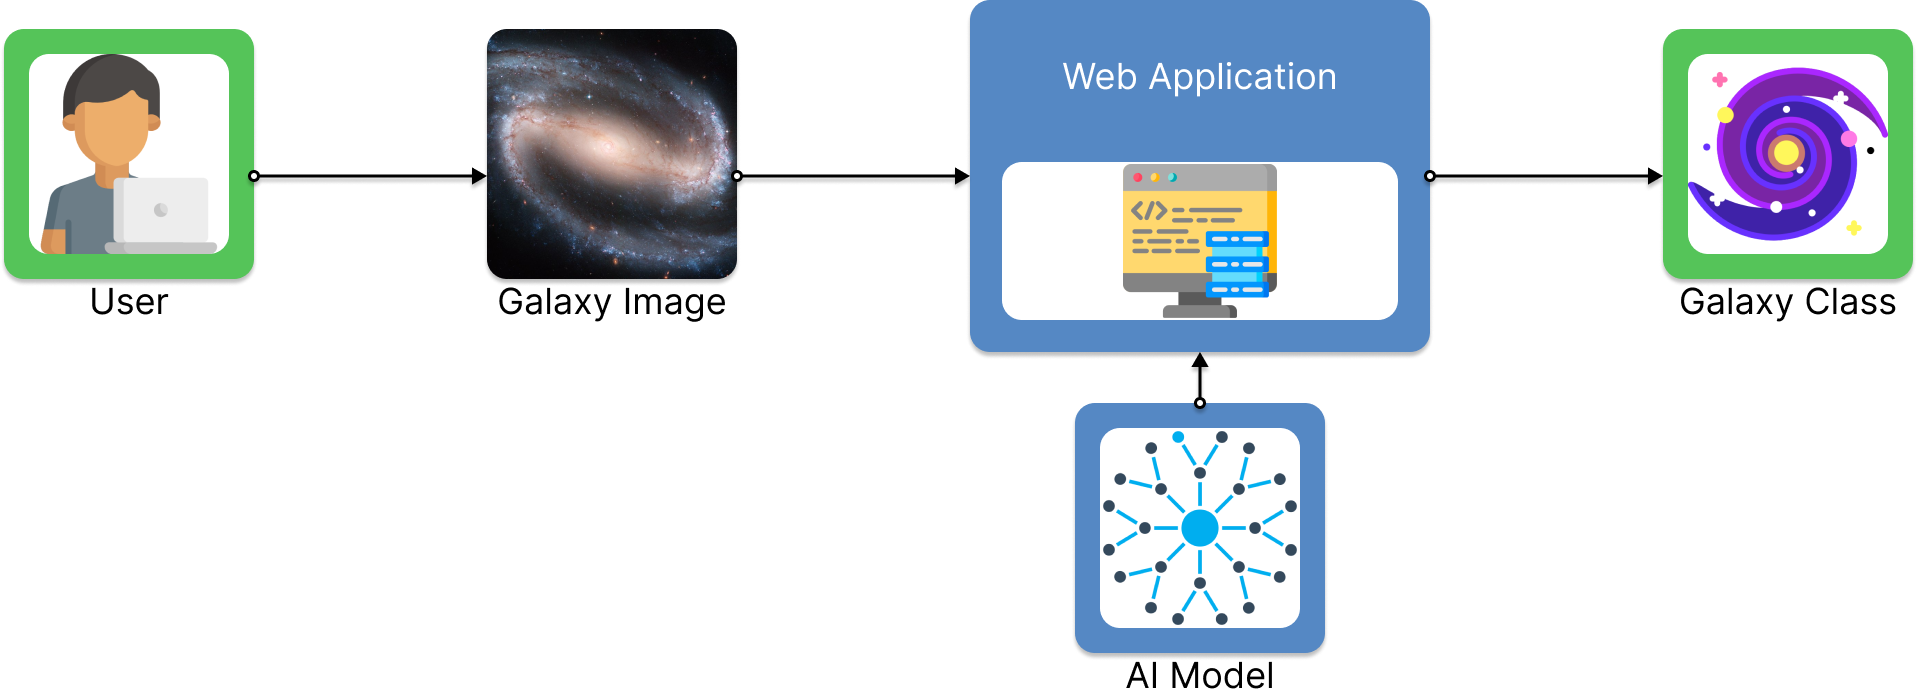
\includegraphics[width=0.8\linewidth]{obrazky-figures/04-draft/idea.png}
  \caption{Illustration of application use case.}
  \label{fig:app-pipeline-user}
\end{figure}

From the user perspective, the application operates via the web without requiring a local installation. The functionality includes uploading galaxy images to obtain their morphology classification, which is determined by an AI model implemented on the backend. From the developers' side, each part of the application should be deployed into cloud-based infrastructure, which will provide high robustness and reliability under the high demand. All this leads us to the following functional and non-functional requirements.

\paragraph{Functional Requirements}

\begin{enumerate}
    \item \textbf{Galaxy Image Classification}: The system will classify galaxy images into predefined morphological categories using a AI model.
    \item \textbf{Model Integration}: The backend will load the model at startup and manage its lifecycle.
    \item \textbf{Scalability}: The system will support horizontal scaling to handle increased load, utilizing Openshift and its Kubernetes-based orchestration.
\end{enumerate}

\paragraph{Nonfunctional Requirements}

\begin{enumerate}
    \item \textbf{Deployment Platform}: The application shall be deployed on the Red Hat OpenShift Container Platform.
    \item \textbf{Performance}: The application will handle multiple concurrent users without significant degradation in performance.
    \item \textbf{Real-time Responsiveness}: The application shall process and return results for any user-initiated action in under 200 ms (0.2 s).
    \item \textbf{Accuracy}: The classification model will achieve competitive accuracy, comparable to existing models in the field
\end{enumerate}

To accomplish this, we must address the following foundational questions: \enquote{How do Artificial Neural Networks function?}, \enquote{Which architecture to use?}, \enquote{How can the dataset be utilized for model training?}, \enquote{What are the features of apps with AI?}, \enquote{What is the process of deploying an AI-based application into a cloud-based platform?}. These questions will be addressed in the following chapters. The result of this exploration is an application developed to apply the latest AI advancements as a practical tool for astronomers to classify galaxy images. The application will illustrate how a fully containerized, real-time service can be deployed on Red Hat OpenShift, balancing resource limitations with model performance.

\chapter{Artificial Neural Networks}
\label{chapter:ann}

As demonstrated in \autoref{sec:modern-app}, AI‑based tools can achieve excellent results. However, before using advanced models, it is necessary to understand how AI works and what advantages Machine Learning offers over traditional AI algorithms. This chapter introduces the fundamentals of artificial neural networks. Following this, we will discuss the details behind AI models' learning process and how they make predictions. Furthermore, a significant emphasis of this chapter is on understanding Vision Transformer architectures.

\section{Machine Learning}

Traditionally, the sophisticated algorithms written by programmers were used to make the systems \enquote{intelligent}. An instance of such an algorithm for detecting the presence of a dog in a photo could be formulated as \enquote{If there are three black circles in a triangular arrangement within an image, it should be identified as a dog.} Nevertheless, this rule would fail against a close-up shot of a muffin:

\begin{figure}[htbp]
    \centering
    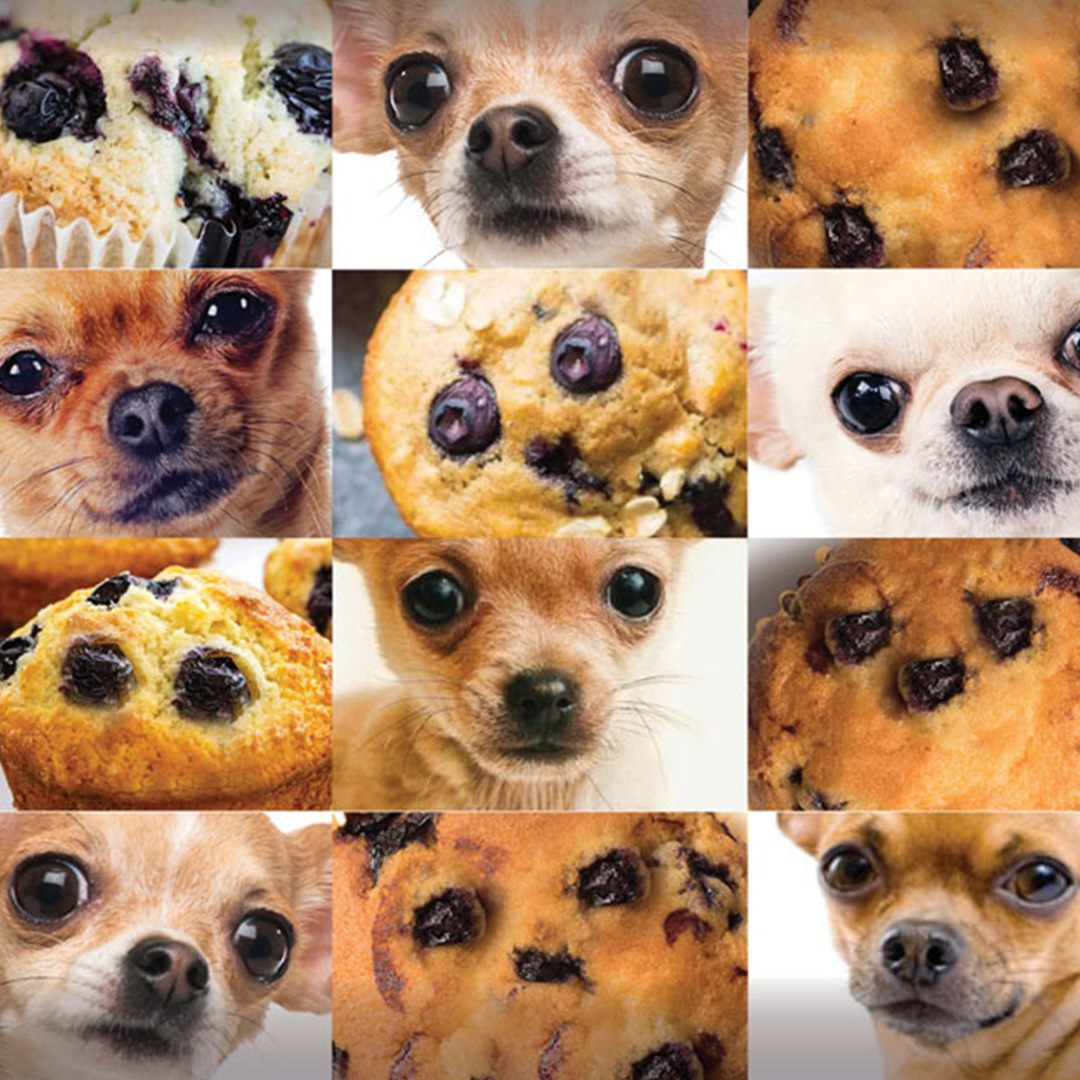
\includegraphics[width=0.5\textwidth]{obrazky-figures/02-theoretical-basis/muffin.jpg}
    \caption{Dogs and Muffins.}
    \label{fig:muffin}
\end{figure}

We can apply the same principle to any field. In the past, if someone was interested in creating a program to solve a practical problem, they needed to understand everything about the input data. The programmer would then write as many rules as possible to cover every possible edge case. Neural networks provide a unique benefit by combining feature extraction with the use of those features for classification or regression. Since it is not needed to come up with rules for classifying images, it eliminates most of the labor associated with traditional techniques for engineers.

Neural networks are not programmed in the traditional sense. They are trained using specific datasets. Their capacity to learn during this training process represents a significant advantage over traditional algorithms \cite{ayyadevara2024modern}. During the training, neural networks are able to identify complex dependencies between input and output data, as well as perform generalization. This means that in case of successful training, the network will be able to provide accurate results even when given data that is missing from the original training dataset, incomplete, or noisy.

\section{ANN Building Blocks}

An artificial neural network (ANN) is a computational model inspired by the structure and function of the brain's neural network. ANNs are designed to recognize patterns and solve complex tasks by processing information in a layered manner, much like how neurons in the brain work to perform cognitive functions.

An ANN is a collection of tensors (weights) and mathematical functions that take in one or more tensors as inputs and predict one or more tensors as outputs. The arrangement of operations that connects these inputs to outputs is referred to as the architecture of the neural network. Such architecture can be customized based on different parameters. For example, whether the problem contains structured (tabular) or unstructured (image, text, and audio) data (which is the list of input and output tensors).

The artificial neural network is composed of interconnected artificial neurons, often called nodes. Each artificial neuron receives inputs from connected neurons or from the input data at the first layer. It then processes inputs by applying weights to them, summing them up, and passing the result to an activation function.

\begin{figure}[htbp]
    \centering
    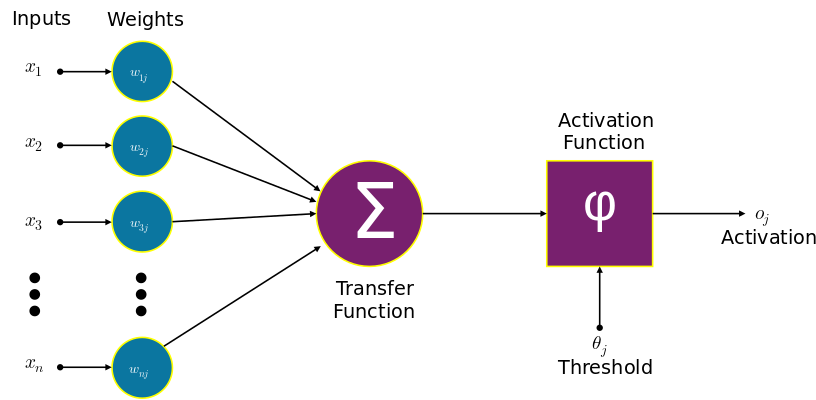
\includegraphics[width=0.8\textwidth]{obrazky-figures/02-theoretical-basis/Artificial_neuron_structure.png}
    \caption{Artificial neuron structure. (\url{https://commons.m.wikimedia.org/wiki/File:Artificial_neuron_structure.svg}).}
    \label{fig:neuron}
\end{figure}

In the \autoref{fig:neuron}, \textit{x1},\textit{x2}, ..., \textit{xn} are the input variables, and \textit{w1j}, ..., \textit{wnj} are the bias weights (similar to the bias in linear regression).
 
An activation function is a mathematical function that determines whether a neuron should be activated. The main goal of the activation function is to introduce a nonlinearity to the network. It determines how the inputs from the previous layer should be transformed and passed to the next layer. Without activation functions, neural networks would behave like simple linear models, limiting their ability to learn the complex relationships in data.

\medskip

Neurons are grouped into layers. We can distinguish several types of layers. Different layers may perform different transformations on their inputs.

\begin{figure}[htbp]
    \centering
    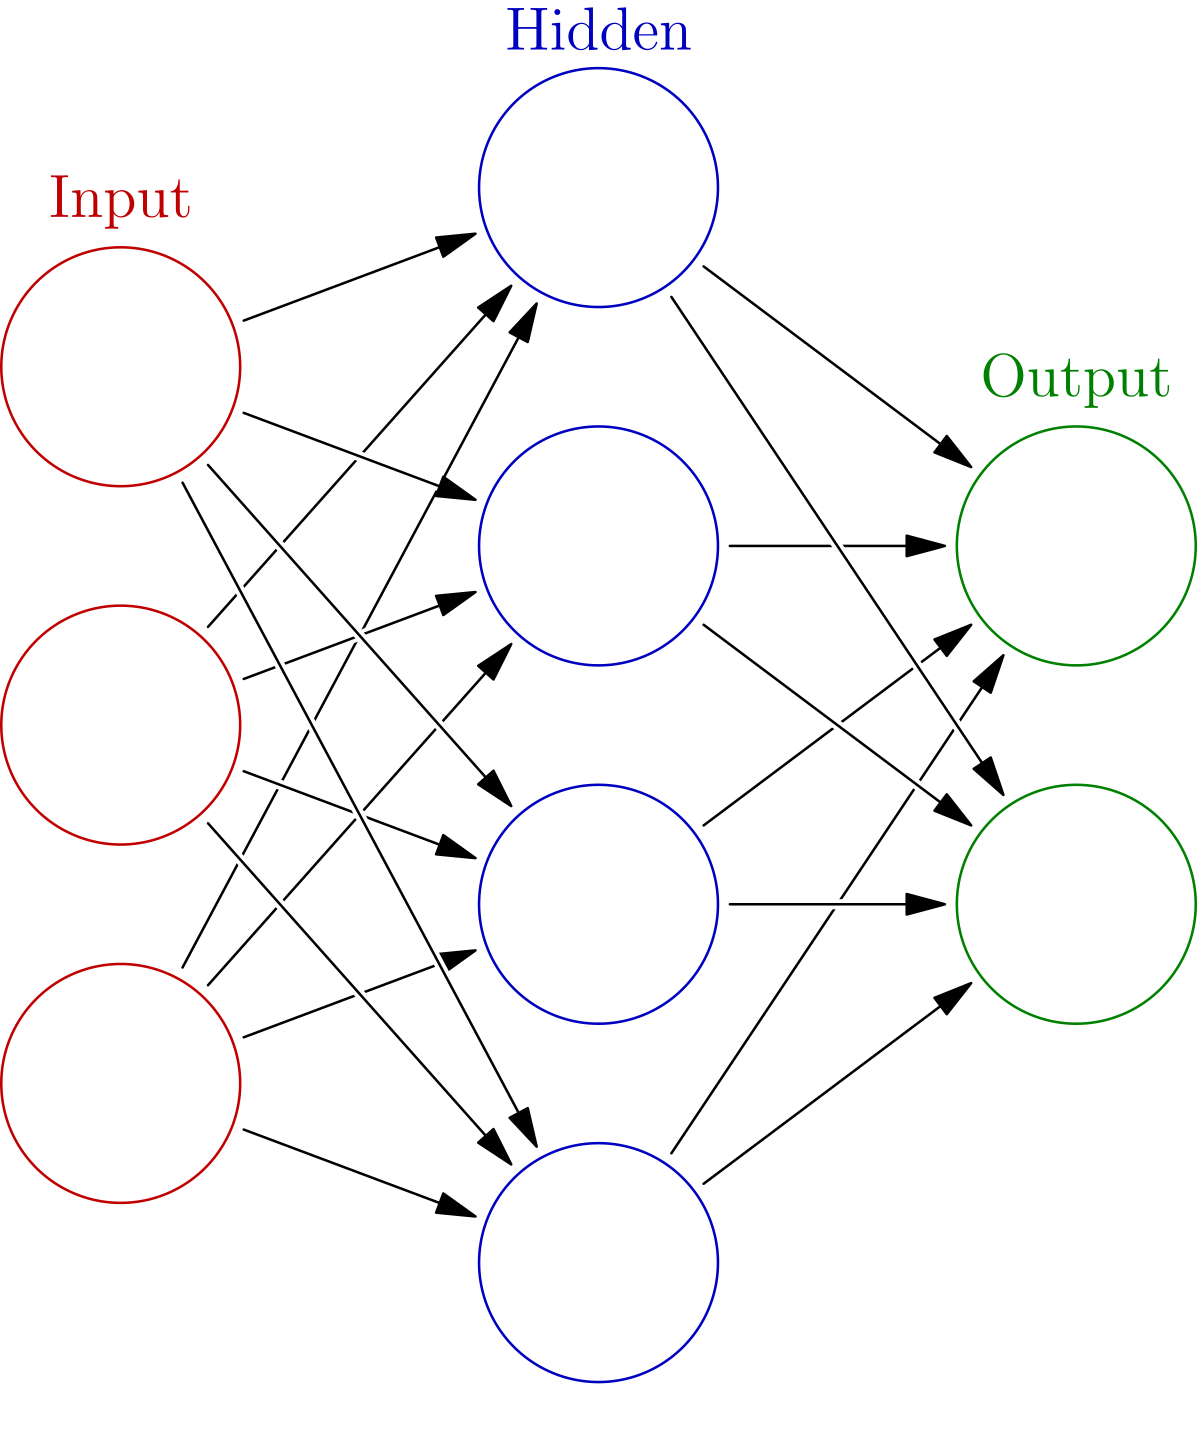
\includegraphics[width=0.45\textwidth]{obrazky-figures/02-theoretical-basis/Colored_neural_network.png}
    \caption{Neural network layers (\url{https://www.researchgate.net/figure/General-structure-of-an-ANN-layer\_fig3\_347819607}).}
    \label{fig:layers}
\end{figure}


The input layer is the first layer of the network. It is responsible for receiving the raw input data. It passes the input features to the next layer in the network and does not perform any computations. The number of neurons in the input layer corresponds to the number of features in the dataset. In scenarios involving image data where each pixel represents an individual feature, the number of neurons within the input layer will correspond to the total number of pixels present in the image.

The hidden layers are the core computational units of an ANN. Hidden layers learn patterns, features, and representations from the data. An artificial neural network can have one or more hidden layers, which are responsible for converting the inputs into internal representations. Architectures incorporating several hidden layers, termed deep neural networks, possess the capacity to discern more complex patterns.

The final layer is called the output layer. Its purpose is to provide the prediction based on the learned patterns from the hidden layers. The number of neurons in the output layer depends on the type of task. For regression tasks that involve predicting a continuous value (like predicting house prices), the output layer usually contains a single neuron. For binary classification tasks (like dog or muffin), the output layer often has one neuron with a sigmoid activation function. For multiclass classification tasks (like categorizing images into multiple classes), the output layer typically has as many neurons as there are classes. The softmax activation function is often used to generate a probability distribution over the classes. The output from this layer is the final prediction of the network, such as a category label or a continuous value.

\section{Deep Learning}

Deep Learning involves the application of large multi-layer artificial neural networks that process continuous representations, similar to the hierarchical structure of neurons in human brains. At present, it stands as the most successful ML methodology, applicable to all ML types, offering improved generalization from limited data and superior scalability for large datasets and computational resources \cite{manning2020ai}.

\begin{figure}[htbp]
    \centering
    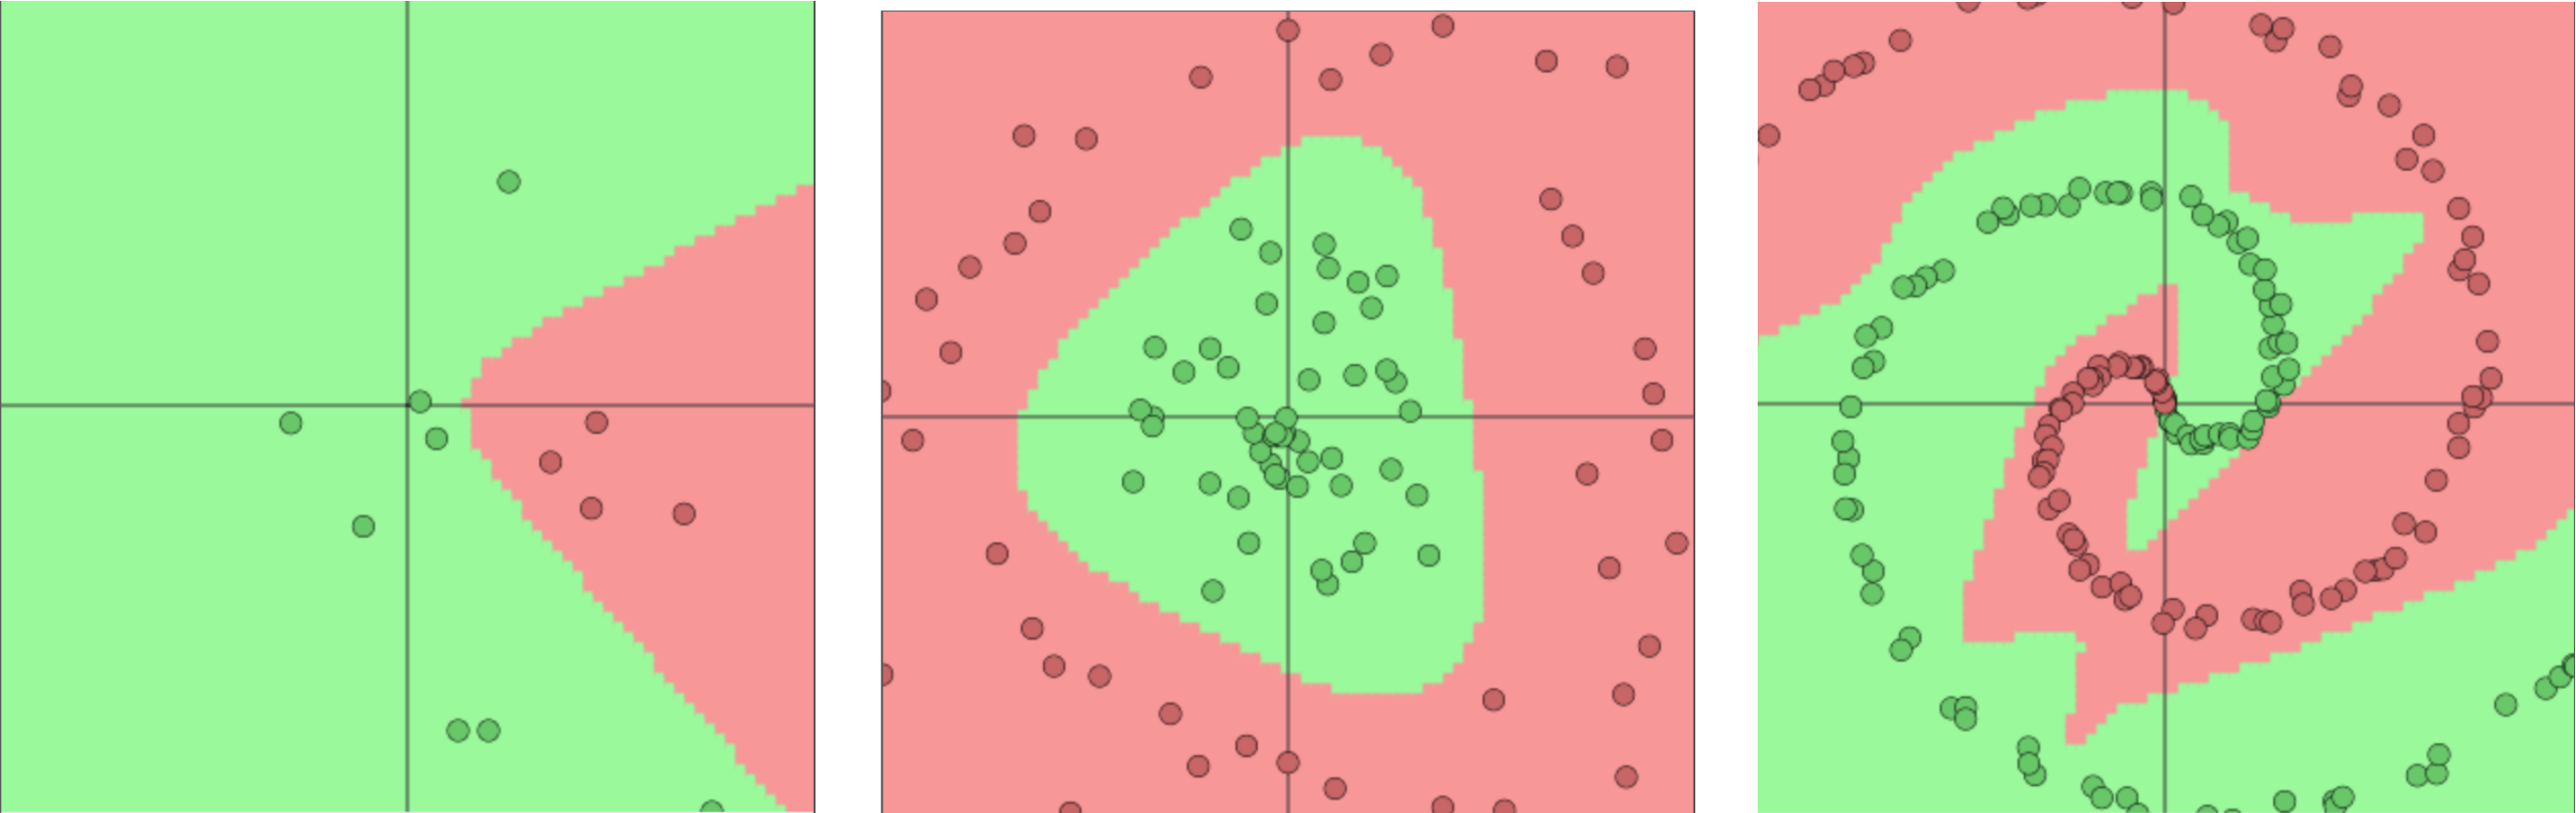
\includegraphics[width=0.8\textwidth]{obrazky-figures/02-theoretical-basis/cnn-ds.png}
    \caption{Space partition for three different data sets. Available at: \url{https://arxiv.org/pdf/1706.00473}.}
    \label{fig:cnn-ds}
\end{figure}

The main difference between Deep Learning and Machine Learning is the structure of the underlying neural network architecture. Deep Learning encompasses a group of models which involve several computational layers. Deep network architectures incorporate nonlinearity in between each layer, which allows a much broader scale of expressivity. Deep Learning, by its nature, is nonlinear and proficient in performing classifications in numerous contexts where linear classification is not sufficient. The majority of contemporary Deep Learning architectures use forward propagation for the computation of outputs and backpropagation for the adjustment of network weights according to error gradients. While a detailed exploration of mathematical formulas is beyond the scope of this thesis, it is important to understand the main meaning of these terms.

A Feedforward Neural Network is a type of artificial neural network where the connections between neurons are directed forward. Unlike recurrent networks, there are no loops or cycles. Data propagates from the input layer through one or more hidden layers to the output layer. For instance, one of the most common feedforward neural networks is a Multilayer Perceptron (MLP). MLP is a type of feedforward neural network consisting of fully connected neurons with a nonlinear kind of activation function. In MLP, neurons process information in a step-by-step manner, performing computations that involve weighted sums and nonlinear transformations.

Backpropagation is a supervised learning algorithm used to train artificial neural networks by minimizing the error between the predicted output and the actual output of the model. The algorithm calculates the gradient of the loss function with respect to each weight by applying the chain rule of calculus, and then updates the weights to reduce the error. Different loss functions can be used for different purposes.

\section{Vision Transformer}

Initially, Convolutional Neural Networks (CNNs) were used for image classification. CNN models can detect image spatial features such as edges, textures, and shapes. This capability is a key factor for object recognition. However, with the evolution of artificial intelligence architectures, fundamentally new methods have been developed. This paved the way for the introduction of a new architecture for image classification known as the Vision Transformer. This architecture applies the attention mechanism, which was originally designed for natural language processing, to visual tasks.

The Vision Transformer (ViT) model was introduced in 2021 in a research paper “An Image is Worth 16*16 Words: Transformers for Image Recognition at Scale” \cite{dosovitskiy2021imageworth16x16words}. Inspired by the success of Transformers in natural language processing, ViT introduces a new way to analyze images by dividing them into smaller patches and leveraging self-attention. This allows the model to capture both local and global relationships within images, leading to high performance in various computer vision tasks.

\subsection*{Original Transformer Architecture}

As the Vision Transformer is based on the Transformer architecture, it is important to take a brief overview of the foundational architecture described in the "Attention Is All You Need" \cite{vaswani2023attentionneed} paper. The mechanism of attention is central across all models within the Transformer family. Understanding the functionality of the Transformer architecture is crucial for leveraging benefits and limitations of the Vision Transformer (ViT) model.

\begin{figure}[htbp]
    \centering
    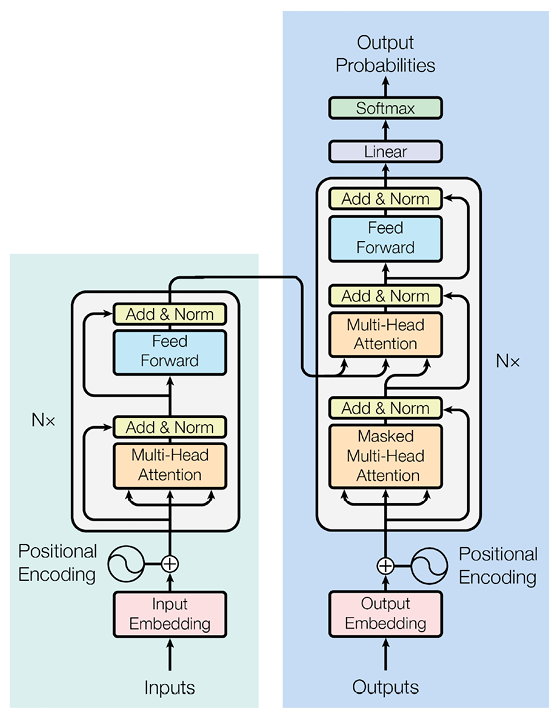
\includegraphics[width=0.55\linewidth]{obrazky-figures/02-theoretical-basis/transformer-architecture.png}
    \caption{Transformer architecture diagram \cite{vaswani2023attentionneed}.}
    \label{fig:transformer_architecture}
\end{figure}


\subsubsection*{Embedding}
Traditionally, textual data in machine learning has been represented as n-gram words. The example of 1-gram: if the original sample has 50,000 unique words, each input sequence would be represented with a 50,000-dimensional vector. We would fill these dimensions with the number of times each word appears in the specific input sequence. However, this approach has several problems. First, even for small input sequences, we require a high-dimensional vector, resulting in a highly sparse vector. Second, there is no meaningful way to perform mathematical operations on these high-dimensional vector representations \cite{timsina2024building}.

Embedding overcomes those challenges. This is a technique used to represent the word or sequence by a vector of real numbers that captures the meaning and context of the word or phrase. An example of embedding is taking a set of words, such as [cabbage, rabbit, eggplant, elephant, dog, cauliflower], and representing each word as a vector in 2-dimensional space capturing animal and color features \cite{timsina2024building}. The embedding representation is shown in \autoref{fig:embedding_plot}.

\begin{figure}[htbp]
    \centering
    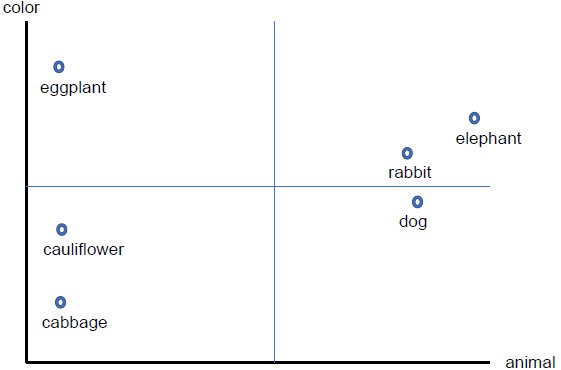
\includegraphics[width=0.7\linewidth]{obrazky-figures/02-theoretical-basis/embedding-vector.png}
    \caption{Embedding plotting \cite{timsina2024building}.}
    \label{fig:embedding_plot}
\end{figure}

The dimension of \enquote{cabbage} and \enquote{cauliflower} is practically identical because both terms refer to vegetables. Consequently, they are positioned close to each other.

\subsubsection*{Positional Encoding}

Positional encoding in a Transformer is used to provide information about the position of each token in the input sequence to the model. Respectively, positional encodings are unique for each position in the sequence. By adding these position-dependent vectors to the input embeddings, the model can distinguish between otherwise identical tokens appearing in different locations. This enables the Transformer to learn not only which tokens to attend to, but also how their relative and absolute positions affect meaning, such as word order in a sentence or spatial relationships in a sequence of image patches.

\newpage
\subsubsection*{Model Input}

The model input is the pointwise addition of the positional encoding and the embedding vector. For example, a tokenized sequence like \enquote{I Live In New York} is shown in \autoref{fig:model_input}.

\begin{figure}[htbp]
    \centering
    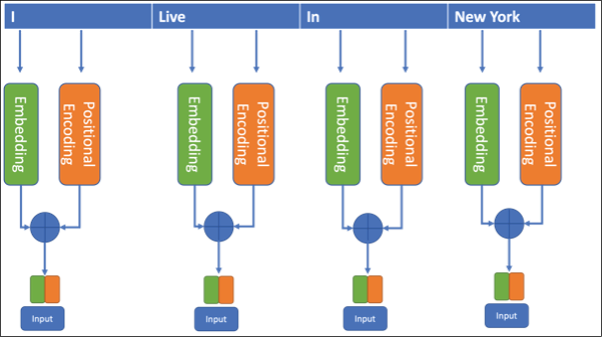
\includegraphics[width=0.7\linewidth]{obrazky-figures/02-theoretical-basis/model-input.png}
    \caption{Model input \cite{timsina2024building}.}
    \label{fig:model_input}
\end{figure}

Each token is represented by an integer. The tokenized sequences are passed to the embedding layer. The embedding of each token is represented by a vector. Finally, the pointwise addition of the embedding and positional encoding is performed before feeding it into the model.

\subsubsection*{Encoder Layer}

The encoder layer is a crucial component in the Transformer architecture, responsible for processing and encoding input sequences into vector representations.

Each encoder block consists of the following components:
\begin{itemize}
    \item \textbf{Input to the encoder:} The input to the first layer of the encoder is the pointwise summation of embeddings and positional encoding.
    \item \textbf{Multi-head attention:} A key component of the encoder block in a Transformer is the multi-head self-attention mechanism. This mechanism allows the model to weigh the importance of different parts of the input when making a prediction.
    \item \textbf{Add and norm layer:} The add layer adds the input to the output of the previous layer before passing it through the next layer. This allows the model to learn the residual function, improving performance. The norm layer normalizes the activations of a layer across all of its hidden units.
    \item \textbf{Feed-forward:} The output of the multi-head attention mechanism is fed to the input of the feedforward layer. A non-linear activation function is applied, and an add-and-norm layer follows it. The output is then fed to the next encoding block.
    \item \textbf{Encoder output:} The last block of the encoder produces a sequence vector, sent to the decoder blocks as features.
\end{itemize}

The encoder produces a sequence vector, which is sent to the decoder blocks.

\subsubsection*{Decoder Layer}
The decoder has a structure similar to the encoder but includes a masked multi-head attention mechanism. The input to the first layer of the decoder is the pointwise summation of the embeddings of the target and the positional encoding of the target sequence.

For the multi-head attention, the decoder receives information from the encoder and previously generated tokens. Also, the decoder uses a masked multi-head attention. Unlike regular multi-head attention, masked multi-head attention prevents the decoder from seeing future tokens. Then, the feedforward layer extracts higher-level features from the data. At the end, the linear layer in the decoder produces the final output, with an activation function generating probabilities for the next word.

\subsubsection*{Attention Mechanism}

The attention is one of the key features that makes the Transformer architecture so successful. The attention mechanism allows models to weigh and prioritize relevant information. There are two main attentions: Self-attention and Multi-headed attention.

\begin{figure}[htbp]
    \centering
    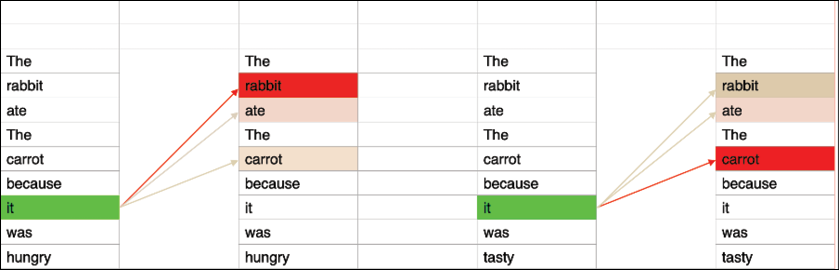
\includegraphics[width=0.99\linewidth]{obrazky-figures/02-theoretical-basis/self-attention.png}
    \caption{Self-attention mechanism \cite{timsina2024building}.}
    \label{fig:self_attention}
\end{figure}

\begin{figure}[htbp]
    \centering
    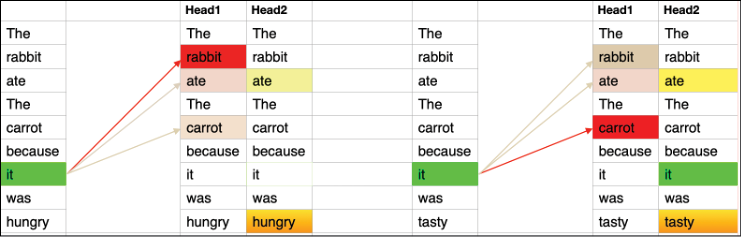
\includegraphics[width=0.99\linewidth]{obrazky-figures/02-theoretical-basis/multi-head-attention.png}
    \caption{Multi-head attention \cite{timsina2024building}.}
    \label{fig:multi_head_attention}
\end{figure}

Self-attention calculates relationships between input tokens to understand their context. \autoref{fig:self_attention} demonstrates how self-attention works, showing how weights are assigned to tokens like \enquote{it} in different sentences. Multi-headed attention uses multiple heads to focus on different features of the input. \autoref{fig:multi_head_attention} illustrates how multiple attention heads capture distinct contextual relationships.

\subsection*{Vision Transformer (ViT) Architecture}

Nowadays, transformers have become the model of choice to perform any task related to natural language processing (NLP). This architecture allows training a model with more than a hundred billion parameters without the need for preliminary model performance saturation. Inspired by the success that transformers achieved when applied to NLP, it was proposed to take advantage of the same architecture in order to perform image classification. The main goal over CNNs was to use the self-attention mechanism that could improve accuracy in image classification tasks.

The authors of \enquote{An Image is Worth 16x16 Words: Transformers for Image Recognition at Scale} \cite{dosovitskiy2021imageworth16x16words} proposed the Vision Transformers (ViT) architecture, which consists of breaking the image into 2D patches and providing this linear sequence of patches as input to the model. A ViT is represented at \autoref{fig:vit-architecture}.

\begin{figure}[htbp]
    \centering
    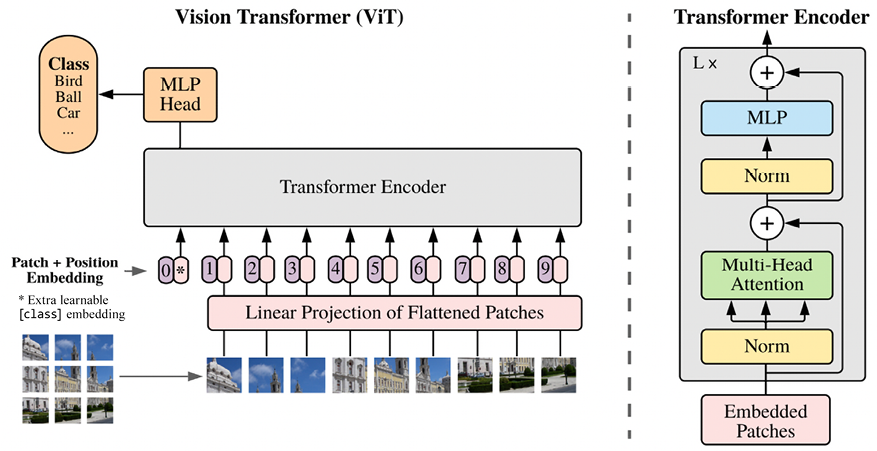
\includegraphics[width=0.8\linewidth]{obrazky-figures/02-theoretical-basis/vit-architecture.png}
    \caption{Vision Transformer architecture \cite{dosovitskiy2021imageworth16x16words}.}
    \label{fig:vit-architecture}
\end{figure}

In Vision Transformers (ViT), the input image is divided into fixed-size patches, similar to how a sentence is split into words in natural language processing tasks. The workflow can be briefly described in the following steps:

\begin{enumerate}
    \item \textbf{Patch Extraction:} The input image is divided into a grid of patches. For instance, if the image size is 300x300, we can extract 9 patches of size 100x100. Each patch is then flattened into a 1D vector.
    \item \textbf{Linear Projection:} Each flattened patch is passed through a linear projection layer to create patch embeddings. This process is analogous to generating word embeddings in NLP, where each patch represents a visual token.
    \item \textbf{Positional Embeddings:} To retain the spatial information of each patch within the image, positional embeddings are added to the patch embeddings. These positional embeddings ensure that the model understands the relative positions of the patches in the original image. Additionally, a special \textit{class token} is introduced, which is used later for classification tasks.
    \item \textbf{Transformer Encoder:} The combined embeddings (patch embeddings + positional embeddings + class token) are fed into the Transformer encoder. Here, the data passes through several layers consisting of multi-head self-attention mechanisms, normalization, and feedforward layers. These layers allow the model to capture both local and global relationships between the patches.
    \item \textbf{Final Classification:} After processing the embeddings, the output corresponding to the \textit{class token} is used for image classification. The embeddings of the remaining patches can also be used as features for other tasks, such as object recognition or image captioning.
\end{enumerate}

\subsection*{Vit and CNN Comparison}
\label{sec:vit-cnn-comparison}

Both Vision Transformers (ViT) and Convolutional Neural Networks (CNN) still remain a popular choice for tasks involving image processing or recognition. However, these architectures represent two different approaches to image classification, each offering unique advantages and limitations. 

\medskip

In this section, CNN and ViT architectures' key components will be compared, including architecture, robustness, efficiency, and scalability. This comparison will provide a clearer understanding of the features of using the Transformer architecture. This is essential for creating an application, which functionality relies on a ViT-based model.

\paragraph{Architecture features}

ViTs use a self-attention mechanism to extract global dependencies across an entire image. Images are split into fixed-size patches, which are treated similarly to tokens in NLP tasks. The self-attention mechanism then allows the model to weigh the importance of each patch relative to others, capturing both local and global context in a single pass. 

In comparison, CNNs have local receptive fields, where each neuron processes only a small region of the image. The global processing capability of ViTs makes them highly effective for tasks requiring context over long distances within an image.

\paragraph{Dataset performance}

ViTs demonstrate superior performance on large datasets due to the self-attention mechanism's ability to capture long-range dependencies and relationships between patches. For smaller datasets, ViTs often require pretraining on larger datasets or extensive data augmentation to outperform CNNs. Studies have shown that ViTs can achieve impressive results in specific applications, such as crop and weed monitoring with UAV images, sometimes achieving higher F1-scores and accuracy compared to CNNs.

\paragraph{Robustness}

Another crucial aspect of comparison between CNNs and ViTs is their robustness to disturbances in images. ViTs have been found to be more robust than CNNs in several tasks due to their ability to model global dependencies across the entire image. This global context allows ViTs to better handle the disturbances in images, such as noise, occlusions, etc. For example, in digital holography, ViTs are able to capture the entire hologram, rather than focusing on localized areas. Moreover, ViTs demonstrate better resilience to high-frequency noise that tends to confuse CNNs.

Conversely, CNNs are more sensitive to small perturbations and adversarial examples, primarily due to their reliance on local feature extraction. The property of convolutional layers can lead to reduced performance in tasks where global context is essential, or where input data is violated. But it is worth noting that recent advancements, such as the introduction of anti-aliasing filters and adversarial training, have improved the robustness of CNNs in some cases.

\paragraph{Computational Efficiency}

In terms of computational efficiency, CNNs are generally more efficient than ViTs, particularly for real-time or resource-constrained applications. CNNs benefit from optimized hardware acceleration, which can handle convolution operations efficiently, allowing for faster training and inference. 

Furthermore, various techniques, such as pruning, quantization, and knowledge distillation, can compress CNNs without significant loss in performance, making them suitable for deployment on devices with limited computational power.

ViTs, while capable of parallel processing due to their patch-based input, often require more computational resources due to the self-attention mechanism. Especially when processing high-resolution images or large datasets. The complexity of self-attention with respect to the input size can lead to significant overhead, limiting the scalability of ViTs in resource-constrained environments. However, ViTs have shown promise in reducing the training time when using pre-trained models or leveraging transfer learning, where they can surpass CNNs in training efficiency.

\paragraph{Generalization}

Generalization is another area where CNNs and ViTs differ. ViTs have been found to generalize better to unseen data, especially when fine-tuned on large datasets. The ability of ViTs to capture global relationships in an image helps them generalize well to tasks with varying input distributions. Pretraining ViTs on large-scale datasets, such as ImageNet, has been shown to significantly improve their generalization capabilities.

In contrast, CNNs generally require larger datasets to achieve similar generalization performance. Their reliance on local feature extraction can hinder generalization when trained on small datasets. However, CNNs perform exceptionally well when fine-tuned on domain specific datasets, such as in medical imaging or object detection tasks.

\subsection*{ViT for Image Classification}

The choice of the architecture is usually determined by the goals of the application and the problems this application solves. As it was defined in \autoref{sec:ai-app}, our application should be capable of classifying galaxy images. In our case, there are the following potential problems: images could be highly compressed and noisy; various rotations have a place to be; new galaxies' images, which wouldn't be present in the training dataset, could also be processed and classified. 

\medskip

The reasons why to choose the ViT for our purposes are the following: First, ViTs can handle images of various sizes and aspect ratios without significant loss of information due to resizing or cropping, making them versatile for different image types. Second, ViTs may outperform CNNs in tasks involving noisy or distorted images. Third, due to their capability to capture global relationships, ViTs have superior generalization to new data.

\subsection*{Modern ViT-based Architectures}

Nowadays, there are many advanced architectures that were created by modification of the original ViT. In this section, we will discuss some of the advanced ViT-based architectures that can be suitable for galaxy morphology classification tasks. 

\subsection*{Convolutional Vision Transformer}

\begin{figure}[htbp]
    \centering
    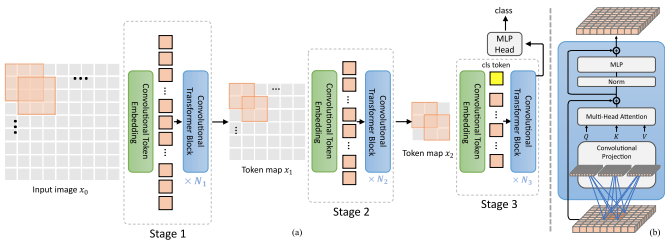
\includegraphics[width=0.8\linewidth]{obrazky-figures/02-theoretical-basis/cvt.png}
    \caption{Convolutional Vision Transformer architecture (\url{https://arxiv.org/abs/2103.15808}).}
    \label{fig:cvt}
\end{figure}

The Convolutional Vision Transformer (CvT) introduces the combination of convolutions with attention mechanisms. The convolutions are utilized to embed and reduce the dimensionality of the image or feature map across three distinct stages. Additionally, depthwise convolution is applied to project the queries, keys, and values for the attention process.

\subsection*{CrossFormer}

\begin{figure}[htbp]
    \centering
    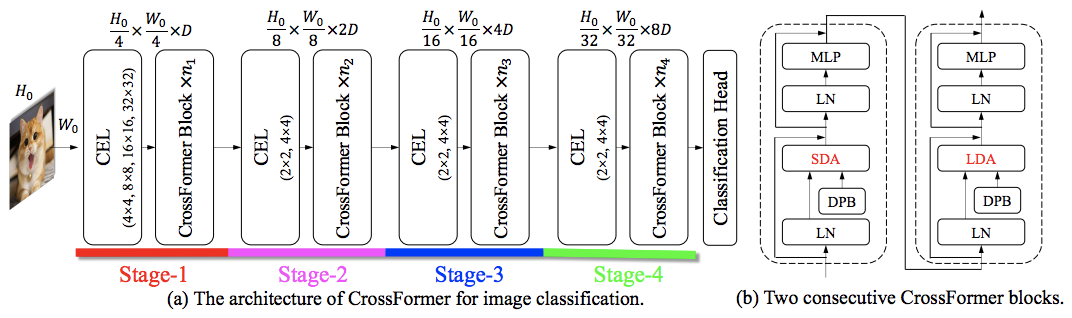
\includegraphics[width=0.8\linewidth]{obrazky-figures/02-theoretical-basis/crossformer.png}
    \caption{CrossFormer architecture \cite{wang2021crossformerversatilevisiontransformer}.}
    \label{fig:crossformer}
\end{figure}

The authors of \enquote{CrossFormer: A Versatile Vision Transformer Hinging on Cross-scale Attention} \cite{wang2021crossformerversatilevisiontransformer} claim that their architecture outperforms PVT and Swin by employing alternating local and global attention mechanisms. The global attention is implemented across the windowing dimension to reduce complexity, similar to the axial attention strategy. They also introduced a cross-scale embedding layer, demonstrated to be a versatile enhancement for all vision transformers. Additionally, a dynamic relative positional bias was developed to enable the network to generalize to images of higher resolutions.

\subsection*{Swin Transformer}

\begin{figure}[htbp]
    \centering
    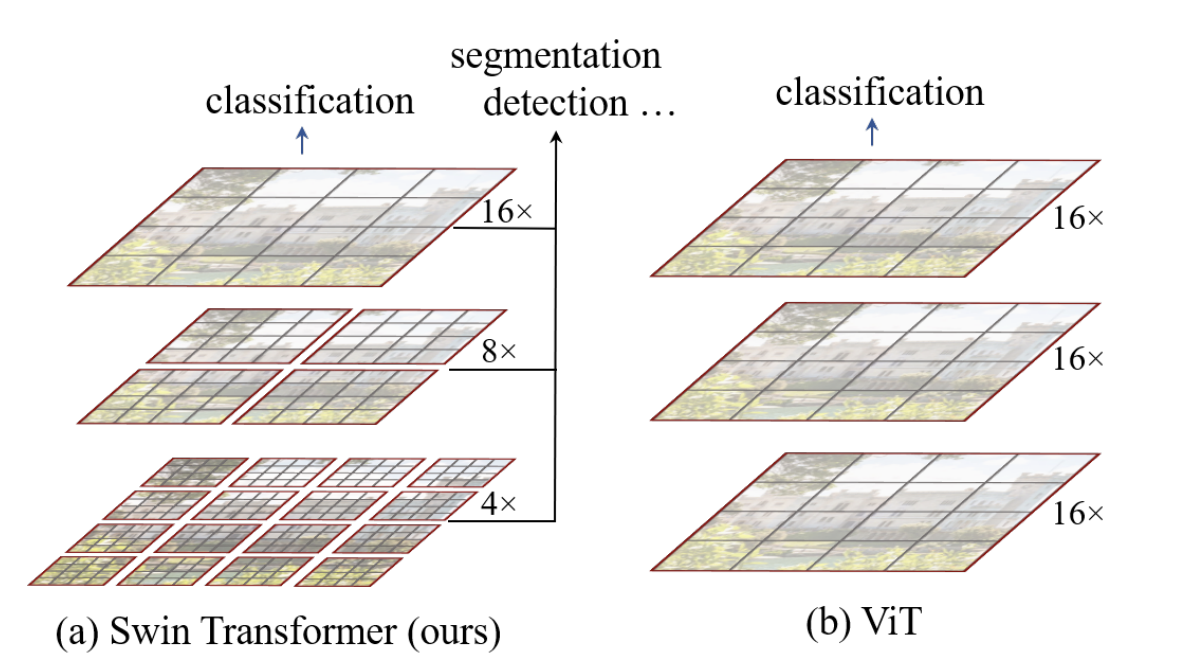
\includegraphics[width=0.5\linewidth]{obrazky-figures/02-theoretical-basis/swin.png}
    \caption{Swin Transformer architecture (\url{https://arxiv.org/pdf/2103.14030v2}).}
    \label{fig:swin}
\end{figure}

The \enquote{Swin Transformer} paper introduces a hierarchical representation approach by splitting the image into separate local windows with no overlaps and performing self-attention within each window. To address cross-window interactions, these windows are shifted in the following layers, aiding in complexity reduction and efficient scaling for bigger images. This architecture delivers robust outcomes across different vision tasks, all while keeping the computational load low.

\medskip

Each architecture can be better than another in certain aspects. The universal approximation theorem says a sufficiently complex neural network can approximate any function. In other words, for any given input, we can design a neural network architecture and tune the weights to predict any arbitrary output. Take any dataset or task; we can design an architecture and fine-tune it until it achieves the desired predictions \cite{ayyadevara2024modern}.

\medskip

For purposes of galaxy classification application, Crossformer architecture has been chosen. The reason is the cross-scale attention design. Galaxy images typically contain large, low-frequency structures (the overall disk or halo) alongside fine, high-frequency details (spiral-arm knots, dust lanes, bar features). CrossFormer’s alternating local–global attention and cross-scale embedding layer let the network model these multi-resolution cues in a single forward pass, improving sensitivity to morphology while keeping the parameters count lower than similarly accurate hierarchical ViTs.

\chapter{Red Hat Openshift}

In \autoref{chapter:ann}, we examined fundamental concepts related to Deep Learning. Nonetheless, one of the most significant challenges associated with AI has not been addressed yet. Although model inference can be run on CPUs, model training is predominantly performed with the use of GPU acceleration. Consequently, a significant amount of VRAM and GPU resources is needed. It could be highly expensive to purchase an AI-dedicated GPU. One of the opportunities to address these problems is using cloud-based computing solutions.

% In this chapter, we will discuss the features of the Red Hat OpenShift AI and OpenShift Container Platform.

\section*{Red Hat Openshift AI Platform}

Red Hat OpenShift AI provides specialized tools and frameworks for data science and machine learning, including an integrated environment to develop, train, deploy, and monitor AI models at scale. At \autoref{fig:red-hat-openshift-ai} the key component of this platform can be seen.


\begin{figure}[htbp]
    \centering
    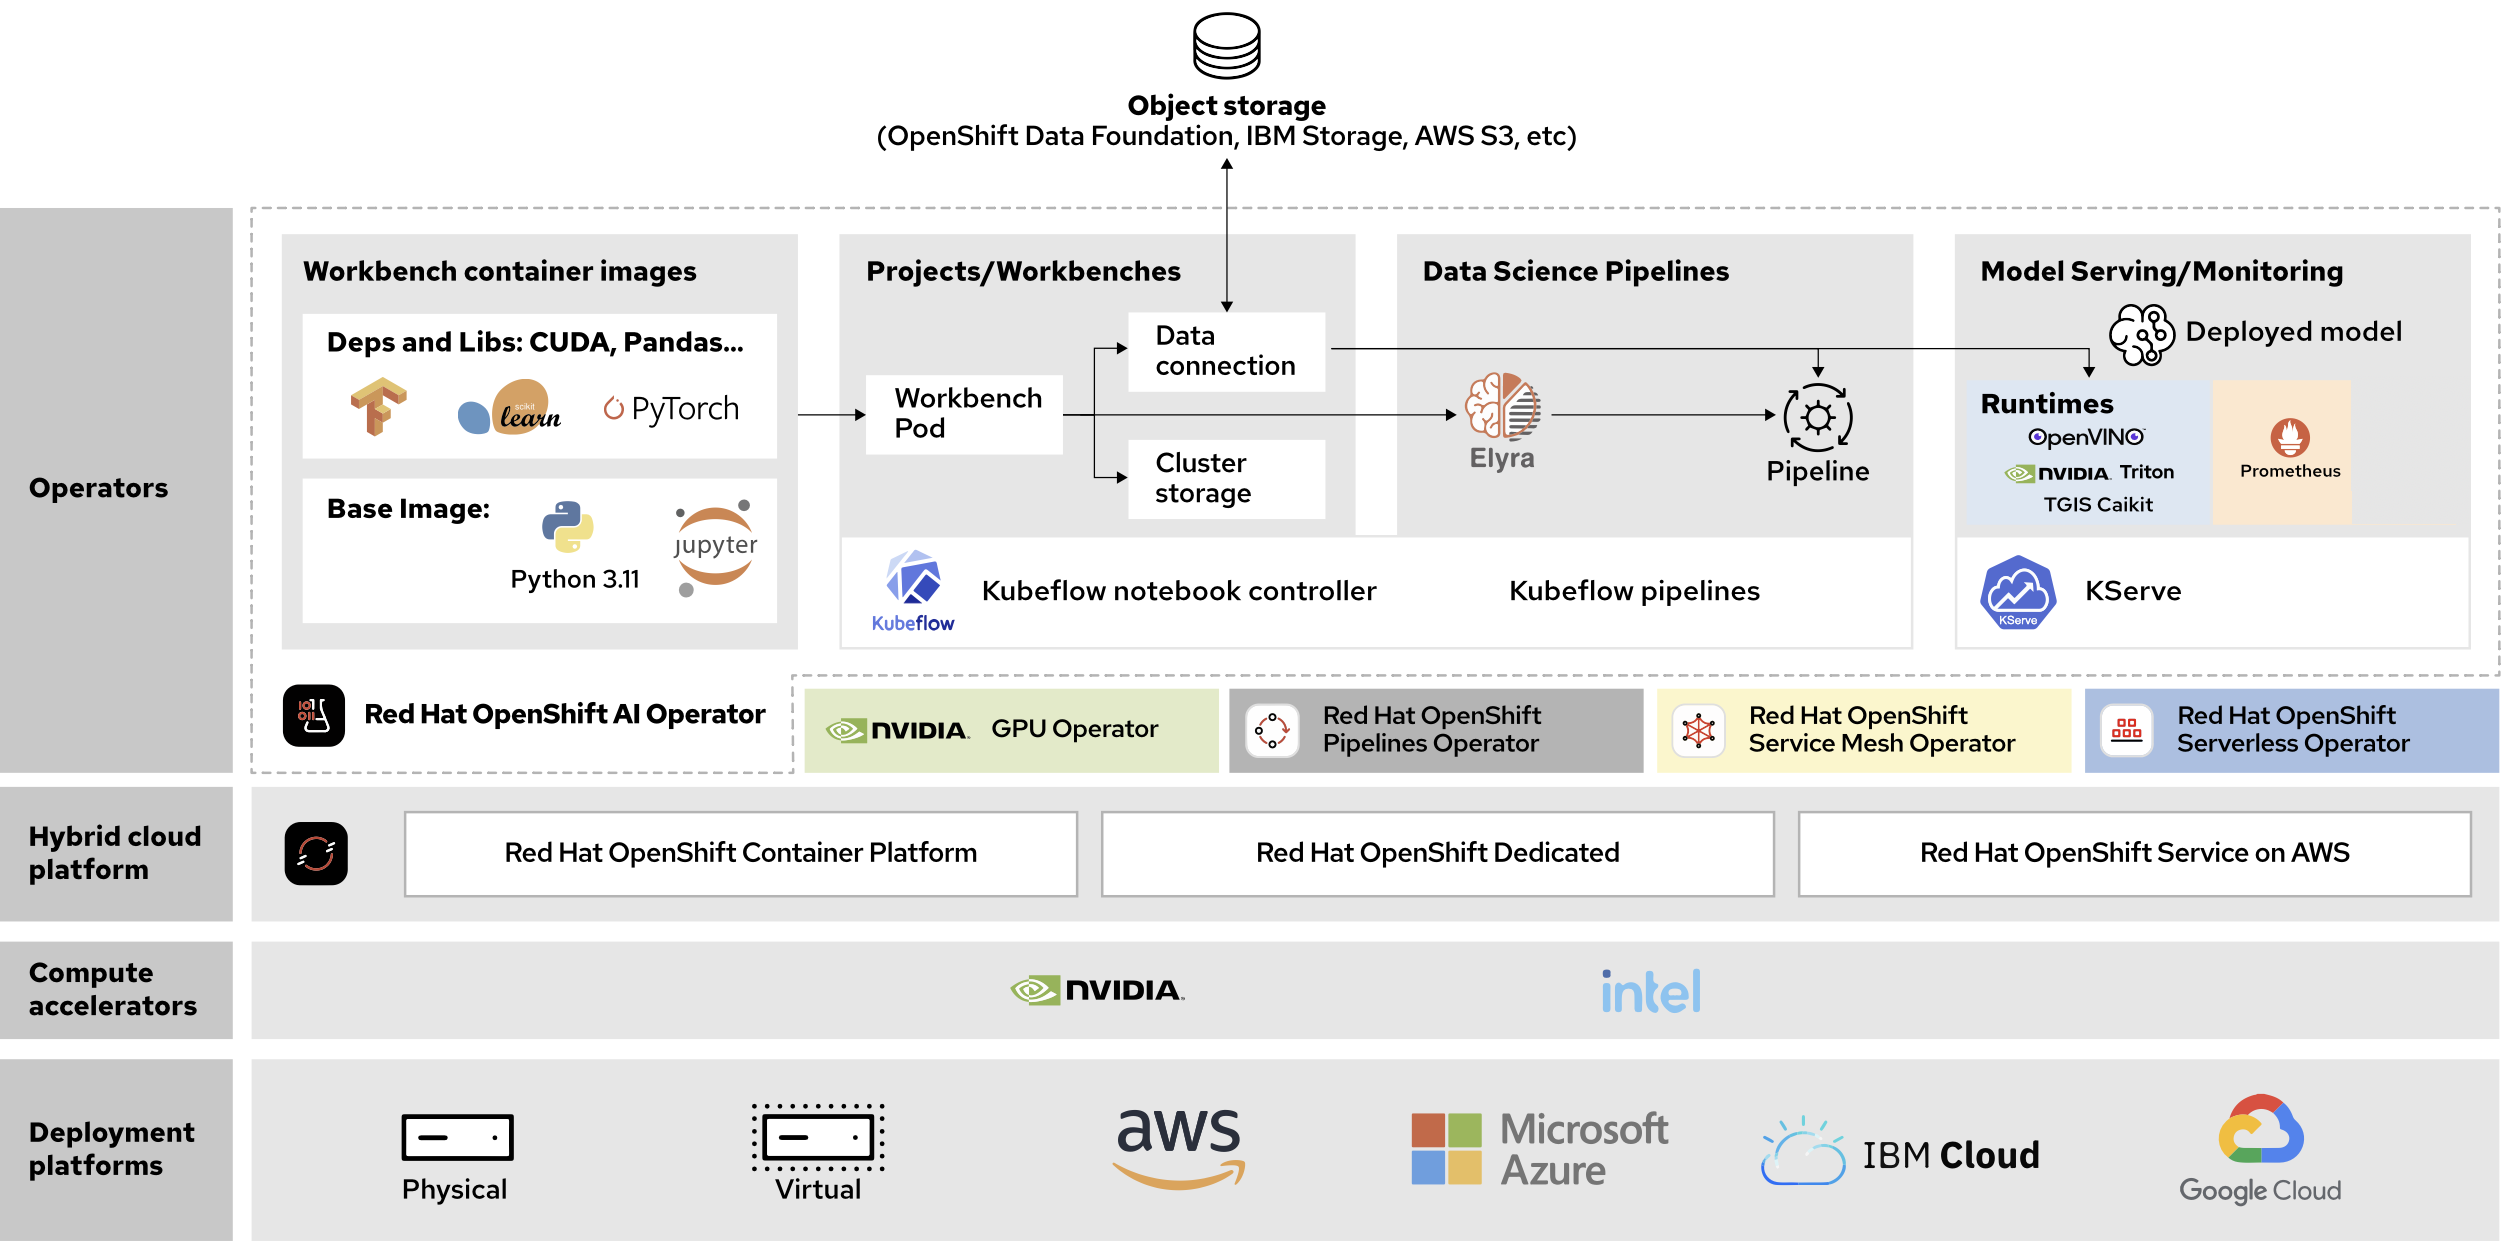
\includegraphics[width=\linewidth]{obrazky-figures/02-theoretical-basis/openshift_ai.png}
    \caption{Architecture of OpenShift AI (\url{https://developers.redhat.com/articles/2024/08/06/red-hat-openshift-ai-and-machine-learning-operations}).}
    \label{fig:red-hat-openshift-ai}
\end{figure}


\textbf{Workbenches}:
In OpenShift AI, a workbench is a containerized environment for data scientists. A workbench image is a container image that OpenShift AI uses to create workbenches. OpenShift AI includes a number of images such as PyTorch, TensorFlow, etc. that are ready to use for multiple common data science stacks. Workbenches run as OpenShift pods and are designed for machine learning and data science. These workbenches include the Jupyter notebook execution environment and data science libraries.

\medskip

\textbf{Cluster storage}:
OpenShift AI uses cluster storage, which is a Persistent Volume Claim (PVC) mounted in a specific directory of the workbench container. This ensures that users will be able to retain their work after logging out or workbench restart.

\medskip

\textbf{Data connections}:
In OpenShift AI, a data connection contains configuration parameters using which you can connect workbenches to S3-compatible storage services.

\medskip

\textbf{Data science pipelines}:
In OpenShift AI, a data science pipeline is a workflow that executes scripts or Jupyter notebooks in an automated way. Using pipelines, it is possible to automate the execution of different steps and store the results.

\medskip

\textbf{Model serving}:
Model server uses a data connection to download the model file from S3-compatible storage. After the download, the model server exposes the model via REST or gRPC APIs. OpenShift AI uses Kserve as the model serving platform and supports model runtimes such as OpenVINO, Triton, Text Generation Inference Server (TGIS), Caikit, etc.

\medskip

\textbf{Model monitoring}:
With the monitoring and logging features provided by OpenShift AI, it is possible to track the performance of the data science workloads and fix any potential problems. 

\medskip

OpenShift AI contains a wide range of tools. For data scientists, OpenShift AI offers a \enquote{Workbench} component. This is an interactive JupyterLab containerized environment that comes with popular libraries and frameworks like TensorFlow and PyTorch. OpenShift AI also supports attaching GPUs or other accelerators to these notebook pods to speed up model training for Deep Learning workloads.

\section*{Red Hat OpenShift Container Platform (OCP)}

Red Hat OpenShift Container Platform (OCP) is a consistent hybrid cloud foundation for building and scaling containerized applications.

OCP provides tools to simplify the application deployment and management by adding extended functionality on top of Kubernetes. One of the main benefits for developers who do not have much experience with Kubernetes is a web console. The web console provides an intuitive GUI that helps users manage resources with no need to use CLI commands. Also, OCP has an integrated CI/CD pipeline, built-in monitoring, and a curated ecosystem of Operators (Kubernetes controllers) for managing services. The platform handles the building, deploying, scaling, and securing containers while letting developers focus on application implementation and maintenance. The core architecture features are illustrated at \autoref{fig:ocp-arch}.

\medskip

In OpenShift, each created object is represented as a declarative resource. These resources are declared as a YAML or JSON manifest, submitted to the API server, and the OpenShift control plane keeps the cluster state with the desired state. So then, the resources needed for deploying a galaxy classification web application will be briefly described below.

\medskip

\textbf{Project} in OpenShift is a Kubernetes namespace enriched with annotations, default network policies, and role-based access control (RBAC) settings. It provides a security-scoped boundary for all of your application’s resources—pods, services, quotas, and so on.

\medskip

\textbf{Deployment} resource declares the desired number of pod replicas running the container image, together with update strategies and liveness/readiness probes. OpenShift uses this to create and manage a ReplicaSet under the covers, ensuring high availability.

\medskip

\textbf{HorizontalPodAutoscaler (HPA)} automatically adjusts the number of pod replicas based on observed metrics (e.g., CPU utilization). This ensures that the classifier scales up under load and scales down to save resources when idle.

\medskip

\textbf{Service} provides a stable network endpoint that load-balances traffic across the pods selected by a label selector. Internally, it allocates a ClusterIP so other pods can discover the classifier backend.

\medskip

\textbf{Route} exposes a Service at a public hostname.

\medskip

\textbf{ResourceQuota} limits the total amount of CPU, memory, and object counts (Pods, Services, Routes, etc.) that can be created in a Project, preventing “noisy neighbors” from consuming all cluster resources.

\medskip

By defining these six resources, OpenShift will maintain the correct number of application pods, automatically scale them with demand, mediate all network traffic, enforce resource budgets, and publish the application at a static URL. This approach permits the treatment of the entire deployment as a unified specification. It should be noted, however, that this does not encompass the entirety of available OpenShift resources. For further details, please refer to the official OpenShift documentation.

\begin{figure}[htbp]
    \centering
    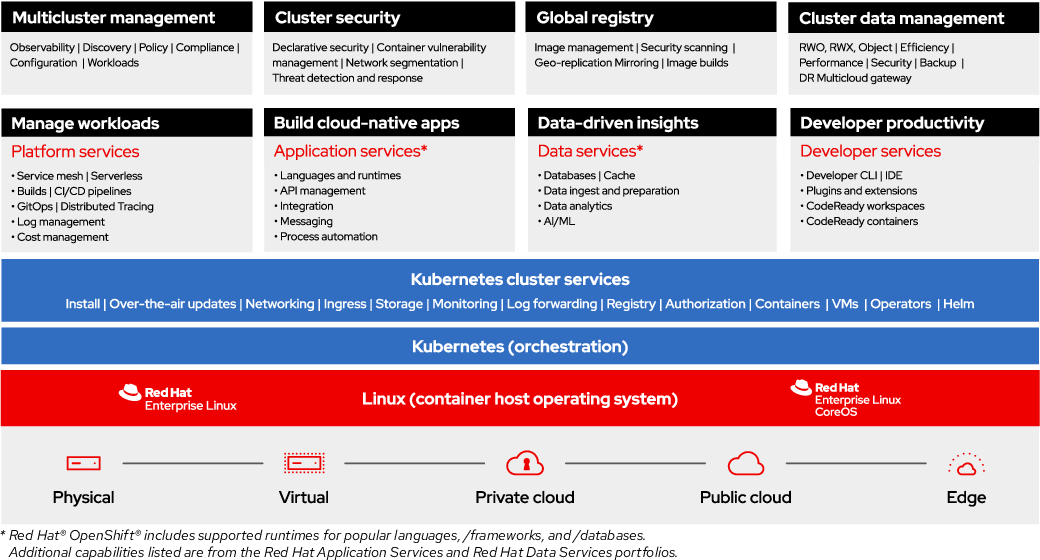
\includegraphics[width=\linewidth]{obrazky-figures/02-theoretical-basis/ocp.png}
    \caption{Architecture of OCP (\url{https://www.redhat.com/en/resources/openshift-container-platform-datasheet}).}
    \label{fig:ocp-arch}
\end{figure}

\chapter{Data and Dataset}
\label{chapter:dataanddataset}

As discussed in \autoref{sec:vit-cnn-comparison}, Vision Transformers (ViTs) necessitate pretraining on larger datasets or extensive data augmentation. The quality of the dataset plays a pivotal role in influencing the accuracy of the model's results. Therefore, this section will be dedicated to the foundational aspects of dataset preparation for model training.

\medskip

Choosing the right dataset is crucial for the success of any machine learning or data analysis task. An accurate and well-structured dataset ensures the model learns meaningful patterns, leading to high accuracy and reliable results. Proper dataset selection can improve generalization, reduce bias, and enhance performance in real-world scenarios. Conversely, using a poorly chosen dataset—such as one with insufficient diversity, outdated information, or mislabeled samples—can result in biased models, overfitting, or inaccurate predictions.

The problem of using an underwhelming dataset can be formulated as \enquote{no matter how well-designed your model or algorithm is, if you train it using poor-quality data, the results will be unreliable.} It can be illustrated by the following figure \autoref{fig:bad-ds}:

\begin{figure}[htbp]
    \centering
    
\includegraphics[width=0.8\linewidth]{obrazky-figures/03-dataset/bad-ds.png}
    \caption{Problem of using underwhelming dataset.}
    \label{fig:bad-ds}
\end{figure}

The very first challenge faced by data scientists involves the identification or creation of a valid dataset suitable for model training. Moreover, in instances where the data lacks variability, it is necessary to develop a comprehensive data augmentation strategy to enhance its resemblance to real-world scenarios.

\section{Galaxy Zoo 2}
\label{sec:gz2-dataset}

Galaxy Zoo 2 (GZ2) extends the original Galaxy Zoo classifications. This is a large-scale, publicly available collection of nearly 300,000 galaxy images sourced primarily from the Sloan Digital Sky Survey (SDSS). It was created as part of the Galaxy Zoo citizen science project, where volunteers classified galaxies based on their morphological features \cite{Willett_2013}.

\begin{figure}[htbp]
    \centering
    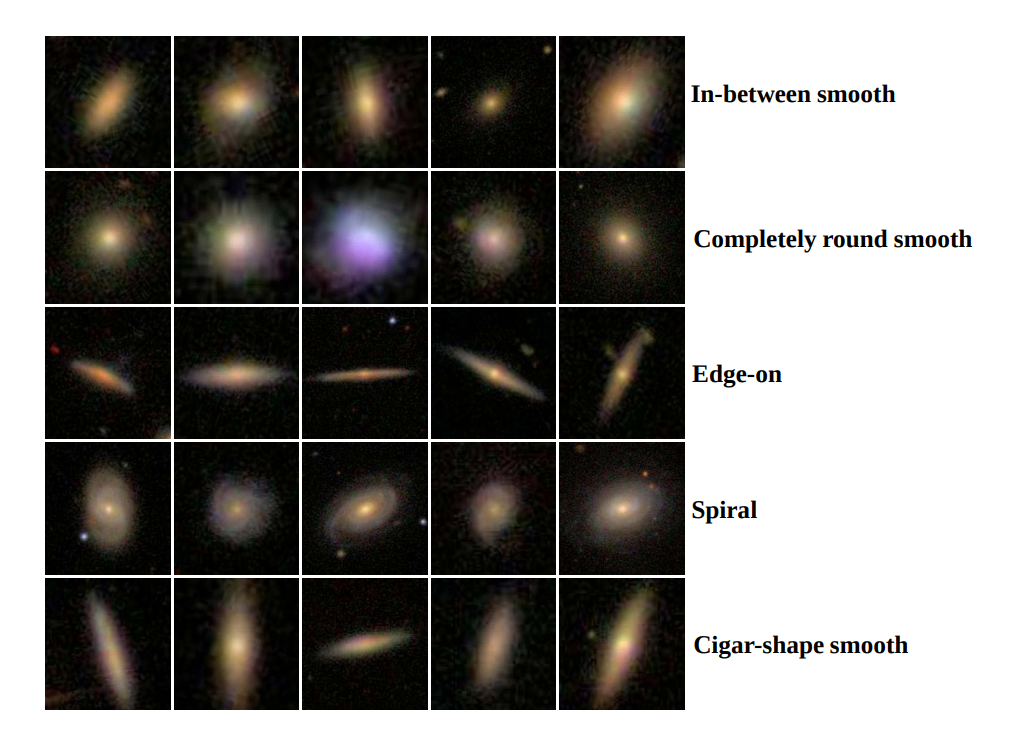
\includegraphics[width=0.6\textwidth]{obrazky-figures/03-dataset/gz2-images.png}
    \caption{Images of galaxy from GZ2. (Source: \href{https://www.aanda.org/articles/aa/full_html/2024/03/aa48544-23/aa48544-23.html\#F2}{Cao, Xu, Deng1, Deng, Yang, Liu and Zhou; "Galaxy morphology classification based on Convolutional vision Transformer (CvT)"}).}
    \label{fig:gz2-images}
\end{figure}

\begin{table}[hbt]
\centering
\renewcommand{\arraystretch}{1.2}
\begin{tabular}{@{}clrrrcr@{}}
\toprule
Class & Sample of Galaxy       & \multicolumn{1}{c}{Train} & \multicolumn{1}{c}{Val} & \multicolumn{1}{c}{Dataset} & \multicolumn{1}{c}{Proportion (\%)} \\ \midrule
0     & In-between smooth      & 7262                      & 807                      & 8069                          & 28                                    \\
1     & Completely round smooth & 7591                      & 843                      & 8434                          & 29                                    \\
2     & Edge-on                & 3513                      & 390                      & 3903                          & 14                                    \\
3     & Spiral                 & 7025                      & 781                      & 7806                          & 27                                    \\
4     & Cigar-shaped smooth    & 520                       & 58                       & 578                           & 2                                     \\ \midrule
      & \textbf{Amount}        & \textbf{25 911}           & \textbf{2879}            & \textbf{28 790}               & \textbf{100}                          \\ \bottomrule
\end{tabular}
\caption{Distribution of galaxy samples across training, validation, and dataset proportions.}
\label{tab:galaxy_samples}
\end{table}

\section{Data Augmentation}
\label{sec:03-data-augmentaiton}

Even though Galaxy Zoo 2 is a robust and mature dataset for AI model training, there are some limitations related to the nature of the astronomical data. Such as imbalance in the number of samples across different classes. This imbalance can distort the training process of any machine learning model, leading it to perform poorly on underrepresented classes. To address this issue, there is a necessity to rebalance the impact of samples within the minority classes by employing data augmentation techniques. For instance, modifying the predicted values of specific classes can be employed. Consequently, errors in predictions concerning minority classes will have a greater influence than errors related to majority classes. This approach contributes to the creation of a more balanced dataset, thereby ensuring that the model acquires sufficient information to effectively discern the distinguishing features of all types of galaxies.

Data augmentation enhances the robustness and generalization capability of the classification model \cite{ayyadevara2024modern}. Galaxies in astronomical images can appear in various orientations and positions depending on the relative positioning of the observation instruments. By applying transformations like rotation and filling empty pixels through nearest-neighbor interpolation, these features can be simulated in the training dataset. This also increases the variance in the data while making the model invariant to such transformations, thereby enhancing its performance on real-world data. Such augmentation is crucial for improving model robustness and generalization, especially when using a ViT-based architecture.

\subsection*{Augmentation Techniques}
\label{sec:augmentation-tech}

There are many different methods of data augmentation that could enhance the dataset. The section below provides a brief introduction to chosen augmentation techniques that are pertinent to the enhancement of galaxy images. A more detailed exploration of the application of those techniques can be found in \autoref{chapter:implementation}.

\medskip


\begin{figure}[htbp]\centering
  \centering
  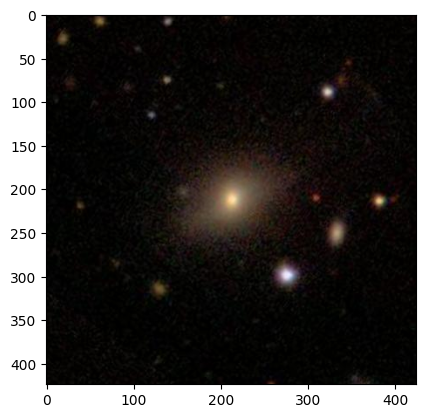
\includegraphics[width=0.5\linewidth]{obrazky-figures/03-dataset/orig.png}
  \caption{Original image sample from dataset}
  \label{fig:orig}
\end{figure}

The sample from the original GZ2 dataset typically represents a photograph of a particular galaxy as shown in \autoref{fig:orig}. The image is centered, has normalized contrast and brightness. The image is quite clear and sharp. Accordingly, each of these aspects can be changed and \enquote{worsened.} In this way, we want to apply augmentation, which will add the distortion inherent in real photos.

\subsubsection*{Resize the image}

First, each model has a certain input window size. That means the images having incompatible sizes will not be processed. So then, it is necessary to resize images so the model can be trained effectively. 

\begin{figure}[htbp]\centering
  \centering
  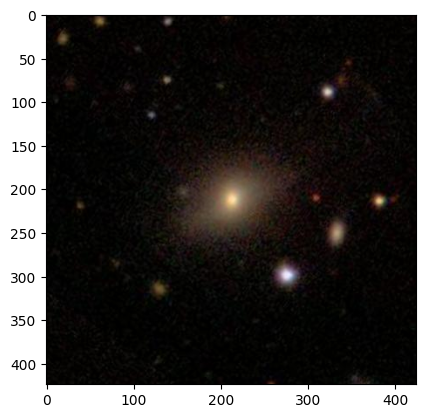
\includegraphics[width=0.5\linewidth]{obrazky-figures/03-dataset/orig.png}\hfill
  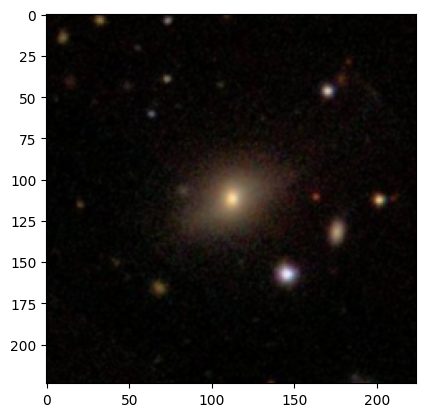
\includegraphics[width=0.5\linewidth]{obrazky-figures/03-dataset/resize.png}
  \caption{Result of image resizing.}
  \label{fig:dataset-sizing}
\end{figure}

The result of resizing is shown at \autoref{fig:dataset-sizing}. Even though images look almost identical, it can be noticed that the left image has a lower resolution.

\subsubsection*{Rotating the image}

Image rotation helps the model to identify the sample in different perspectives and orientations. Allying rotation randomly and on-the-fly helps to ensure that the model will learn the image features rather than the appearance. The result of rotation is shown at \autoref{fig:dataset-rotation}.

\begin{figure}[htbp]\centering
  \centering
  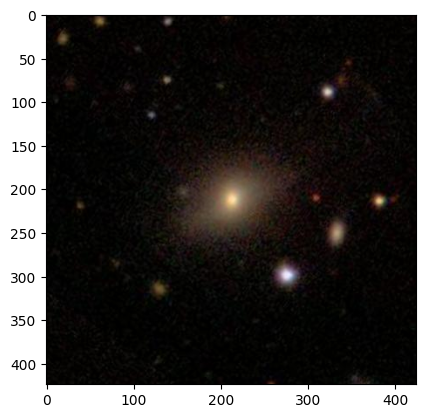
\includegraphics[width=0.5\linewidth]{obrazky-figures/03-dataset/orig.png}\hfill
  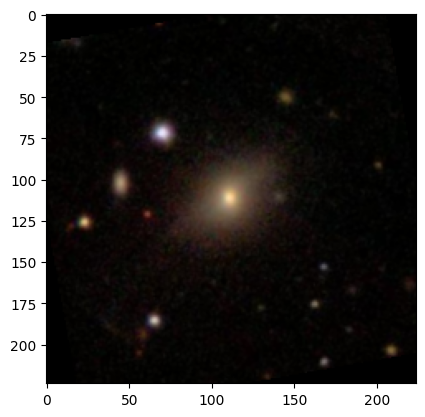
\includegraphics[width=0.5\linewidth]{obrazky-figures/03-dataset/rotation.png}
  \caption{Result of image rotation.}
  \label{fig:dataset-rotation}
\end{figure}

\subsubsection*{Crop}

Cropping images simulates the scenarios when a certain part of the image is not present. It could happen due to image damage or bad image centering by the user. So, it is necessary to make sure the model can extract the features and predict the image class by processing the incomplete image of the galaxy. The cropped image is shown at \autoref{fig:dataset-crop}.

\begin{figure}[htbp]\centering
  \centering
  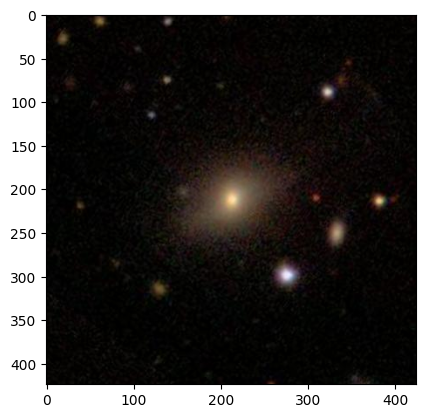
\includegraphics[width=0.5\linewidth]{obrazky-figures/03-dataset/orig.png}\hfill
  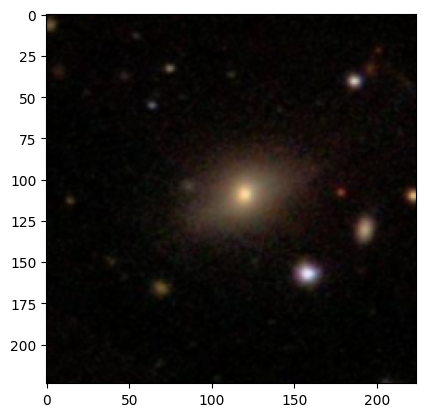
\includegraphics[width=0.5\linewidth]{obrazky-figures/03-dataset/crop.png}
  \caption{Result of image cropping}
  \label{fig:dataset-crop}
\end{figure}

\subsubsection*{Gaussian Blur}

Gaussian Blur applies a low‐pass filter to the image by convolving it with a Gaussian kernel. This operation simulates unfocus or mild blur, ensuring the model learns to recognize objects even when fine details are smoothed.

\begin{figure}[htbp]\centering
  \centering
  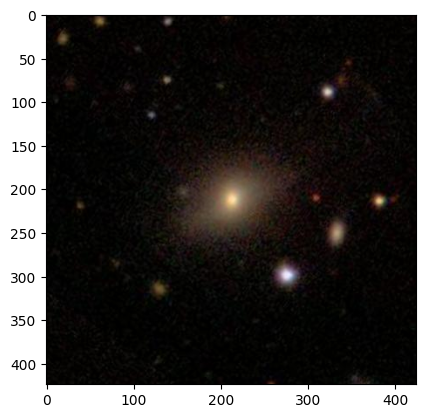
\includegraphics[width=0.5\linewidth]{obrazky-figures/03-dataset/orig.png}\hfill
  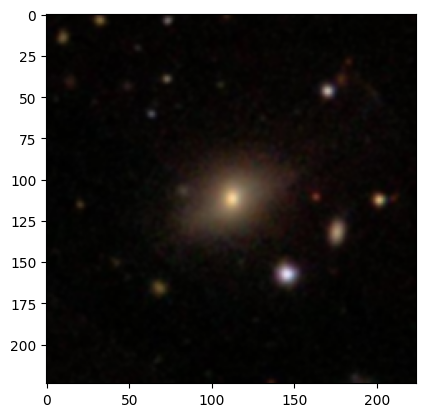
\includegraphics[width=0.5\linewidth]{obrazky-figures/03-dataset/blur.png}
  \caption{Result of applying Gaussian Blur.}
  \label{fig:dataset-blur}
\end{figure}

Applying Gaussian Blur to one leads to a softer appearance and reduced sharpness. This forces the model to learn structural features rather than pixel-level artifacts. The result of applying Gaussian blur is shown at \autoref{fig:dataset-blur}.

\subsubsection*{Color Jitter}

Color Jitter changes the colors of the image. It adjusts the image's brightness, contrast, and colors. Applying this augmentation on-the-fly helps the model learn the same sample in different light and contrast balances. The model learns to predict the image class by shapes rather than just the colors. Color Jitter is illustrated at \autoref{fig:dataset-jitter}.

\begin{figure}[htbp]\centering
  \centering
  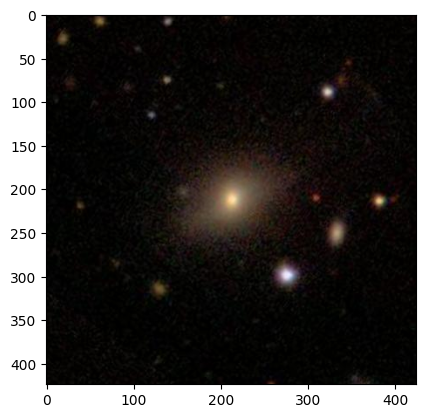
\includegraphics[width=0.5\linewidth]{obrazky-figures/03-dataset/orig.png}\hfill
  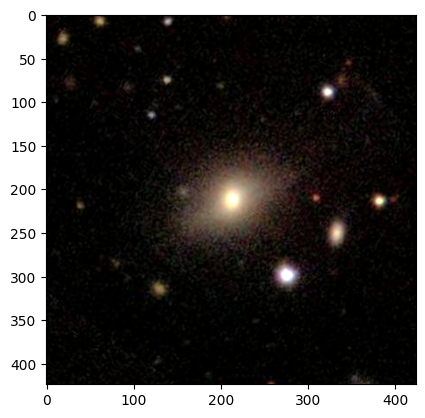
\includegraphics[width=0.5\linewidth]{obrazky-figures/03-dataset/jitter.png}
  \caption{Result of applying color jitter.}
  \label{fig:dataset-jitter}
\end{figure}

The usage of various data augmentation techniques, such as resizing, rotation, cropping, Gaussian blur, and color jitter, serves two main purposes. First, it helps to reduce class imbalance by introducing more realistic variations of existing galaxy images for under-represented categories. Second, it improves model robustness and generalization by adding different image scales, orientations, completeness, and image qualities into the original dataset. Together, these techniques ensure that the ViT-based model will learn essential morphological features of galaxies instead of overfitting to specific imaging pixel-level conditions.

\chapter{Application Draft}

As outlined in \autoref{chapter:core-idea}, the idea behind the application is to translate the recent advances of artificial intelligence into a practical tool that astronomers can easily use for galaxy image classification without installing any software locally. The application should process uploaded photos of galaxies and predict the galaxy's morphology class by using an AI model.

A detailed implementation draft is indispensable before writing a single line of code. It is essential for turning a research prototype into a dependable service. This chapter therefore consolidates every major technical decision from dataset augmentation libraries to cloud deployment. So, the implementation process can proceed systematically, with an understanding of goals, constraints, and expected outcomes.

The Python programming language has become a standard in many fields such as astronomy, data science, and machine learning. A vast collection of well-matured libraries has made this language an obvious choice for researchers and developers. Consequently, this will affect the subsequent choices of technology stack.

\section*{Dataset}
\label{sec:dataset_acquisition}

A well-curated and representative dataset is key to successful and accurate AI-based applications. As mentioned in \autoref{chapter:dataanddataset}, in this work the Galaxy Zoo 2 (GZ2) survey will be used for AI model training. GZ2 is a collection of galaxy images accompanied by detailed morphological labels. There are several options to obtain and use the GZ2 dataset.

\medskip

\textbf{Official Galaxy Zoo web-site}:
The official web site provides the dataset in CSV, FITS, and VOTable formats to download\footnote{Available at: \url{https://data.galaxyzoo.org/}}.
While this format provides an image and labels mapping, it requires manual scripting to reconcile image files with the corresponding labels.

\medskip

\textbf{Hugging Face \texttt{datasets}}:
A pre-packaged version of GZ2 is available through the \texttt{datasets} Python package\footnote{Available at: \url{https://huggingface.co/datasets/mwalmsley/gz2}}. It also requires access to a Hugging Face account to access and use the data.

\medskip

\textbf{Kaggle web-site}:
Kaggle provides an archive that contains the image of each galaxy as well as a csv file with labels mapping\footnote{Available at: \url{https://www.kaggle.com/datasets/jaimetrickz/galaxy-zoo-2-images}}. However, the number of labels is reduced to three: \texttt{objid}, \texttt{sample} and \texttt{asset\_id}. This constraint makes this dataset hard to use for supervised learning.

\medskip

\textbf{Python \texttt{galaxy-datasets} package}:
Finally, the \texttt{galaxy-datasets} provides both imagery and metadata in a single \verb|pip| package\footnote{Available at: \url{https://github.com/mwalmsley/galaxy-datasets}}. Using this package, the data can be downloaded in the format of train and test catalogs. Every catalog is represented as \texttt{pandas.DataFrame}. The provided feature labels include \texttt{summary}, which delineates the galaxy morphology class.

\medskip

Considering the ease of installation and use, \texttt{galaxy-datasets} will be used as a base provider of the GZ2 dataset. The data from this package can be used as \texttt{pandas.DataFrame} for further dataset modifications.

\subsection*{Dataset Repartition}
\label{sec:draft-dataset}

While the \texttt{galaxy-datasets} package offers a convenient solution, it contains only train and test catalogs. However, to ensure that the final accuracy score remains unaffected, it's crucial to separate these into distinct training, validation, and test datasets. The training set will contain images and labels used for model training. The validation set will be used to track accuracy between training epochs. Finally, the test set will remain untouched until the end of training, so the final accuracy will not be biased by any means.

For such dataset modifications \texttt{scikit-learn} Python package will be used. The features of \texttt{scikit-learn} the library are much wider, including classification, regression, and clustering algorithms. Nevertheless, it is ideally suited to meet our requirements.

To utilize dataset augmentation strategies as referenced in \autoref{sec:augmentation-tech}, the \textit{PyTorch} framework is chosen. It offers a huge variety of augmentation techniques available within the \texttt{torchvision.transforms} module.

\section*{AI Model}

Similar to the dataset, there are various ways to acquire the CrossFormer-based model. One option is to build the model from scratch. However, in this thesis, the \texttt{vit-pytorch} Python package will be utilized for model creation. The \texttt{vit-pytorch} package offers ready-made versions of popular ViT-based models implemented using the \texttt{PyTorch} framework.

Correspondingly to model implementation, \texttt{PyTorch} framework can be used for the model training. PyTorch provides a wide range of tools for machine learning, including built-in loss functions (e.g., CrossEntropyLoss and MSELoss), flexible optimizers (such as SGD and Adam), and seamless GPU acceleration. It also includes \texttt{Dataset} and \texttt{DataLoader} classes to encapsulate the process of fetching the data from storage and exposing it into the training loop in batches. The biggest advantage is that employing PyTorch simplifies each phase of model creation and training. The training process of the model will be deployed on the Red Hat OpenShift AI platform.

\section*{Backend}
\label{sec:draft-be}

The backend will be implemented in the Python programming language, known for its extensive use in machine learning applications. The PyTorch library will be utilized for model loading and applying inference tasks. This approach ensures consistency with the AI model built in PyTorch and simplifies the development process.

The backend will establish a (REST) API for communication with the frontend, employing the \texttt{FastAPI} framework. \texttt{FastAPI} is a modern, high-performance web framework designed to create APIs. As for the web server, \texttt{Uvicorn} will be employed. It operates using a multi-process setup, where a primary process manages a pool of worker processes and assigns incoming HTTP requests accordingly.

\section*{Frontend}
\label{sec:draft-fe}

The frontend will be implemented in the JavaScript programming language, using the \texttt{React} library to build modular, reusable UI components. Local development will be based on using Vite, which provides hot-reloading and optimizes bundling for production.

Static assets (HTML, JavaScript, CSS, images) will be served by the \texttt{NGINX} web server. \texttt{NGINX} will deliver cached, versioned front-end bundles directly to clients and also act as a reverse proxy, forwarding any requests under \texttt{/api/} location to the backend service. 

\section*{Red Hat OpenShift}

The application is designed for seamless deployment on modern hybrid-cloud platforms such as Red Hat OpenShift Container Platform. Backend and frontend components will be packaged as Docker images and hosted on Quay.io under the \texttt{rhit\_asultano} namespace. OpenShift Deployments will pull these images at deploy time, ensuring that both services run the exact code that will be developed and tested locally.

All Kubernetes-style resource manifests live in the \texttt{openshift/} folder:

\begin{itemize}
  \item \textbf{Deployments}
    \begin{itemize}
      \item \texttt{cosmoformer-backend-deployment}: defines the Pod template for the FastAPI backend image.
      \item \texttt{cosmoformer-frontend-deployment}: defines the Pod template for the React frontend image.
    \end{itemize}

  \item \textbf{HorizontalPodAutoscalers}
    \begin{itemize}
      \item \texttt{cosmoformer-backend-hpa}: monitors metrics and scales the backend between defined min/max replicas.
      \item \texttt{cosmoformer-frontend-hpa}: similarly scales the frontend based on load.
    \end{itemize}

  \item \textbf{Services}
    \begin{itemize}
      \item \texttt{cosmoformer-backend-service}: exposes the FastAPI Pods internally (ClusterIP) for in-cluster communication.
      \item \texttt{cosmoformer-frontend-service}: exposes the React Pods internally so the Route can direct external traffic.
    \end{itemize}

  \item \textbf{Route}
    \begin{itemize}
      \item \texttt{cosmoformer-frontend-route}: maps an external hostname to the frontend Service, handling TLS and load-balancing. Frontend calls under \texttt{/api/} are proxied to the backend Service.
    \end{itemize}

  \item \textbf{ResourceQuota}
    \begin{itemize}
      \item \texttt{cosmoformer-rq}: enforces CPU, memory, and object-count limits within the project to prevent resource over-usage on the shared (multi-tenant) cluster.
    \end{itemize}

  \item \textbf{Example Project (commented out)}
    \begin{itemize}
      \item \texttt{cosmoformer-app}: a sample of project manifest.
    \end{itemize}
\end{itemize}

By leveraging liveness and readiness probes to automatically detect and replace unhealthy containers, containerized deployment provides robust performance and seamless recovery from failures. Horizontal Pod Autoscaling adjusts the capacity of pods under high load. While Services provide in-cluster connectivity between backend and frontend, Route manages incoming traffic and makes it secure.

This architecture results in a highly resilient and dynamically scalable cloud-native application that can be run in on-premises and public cloud OpenShift environments.

\section*{Final overview}

After a thorough examination and explanations of the primary technical decisions, we can summarize the steps into the unified implementation pipeline for the galaxy morphology classification application. This comprehensive pipeline is illustrated by \autoref{fig:pipeline}:

\begin{figure}[htbp]
  \centering
  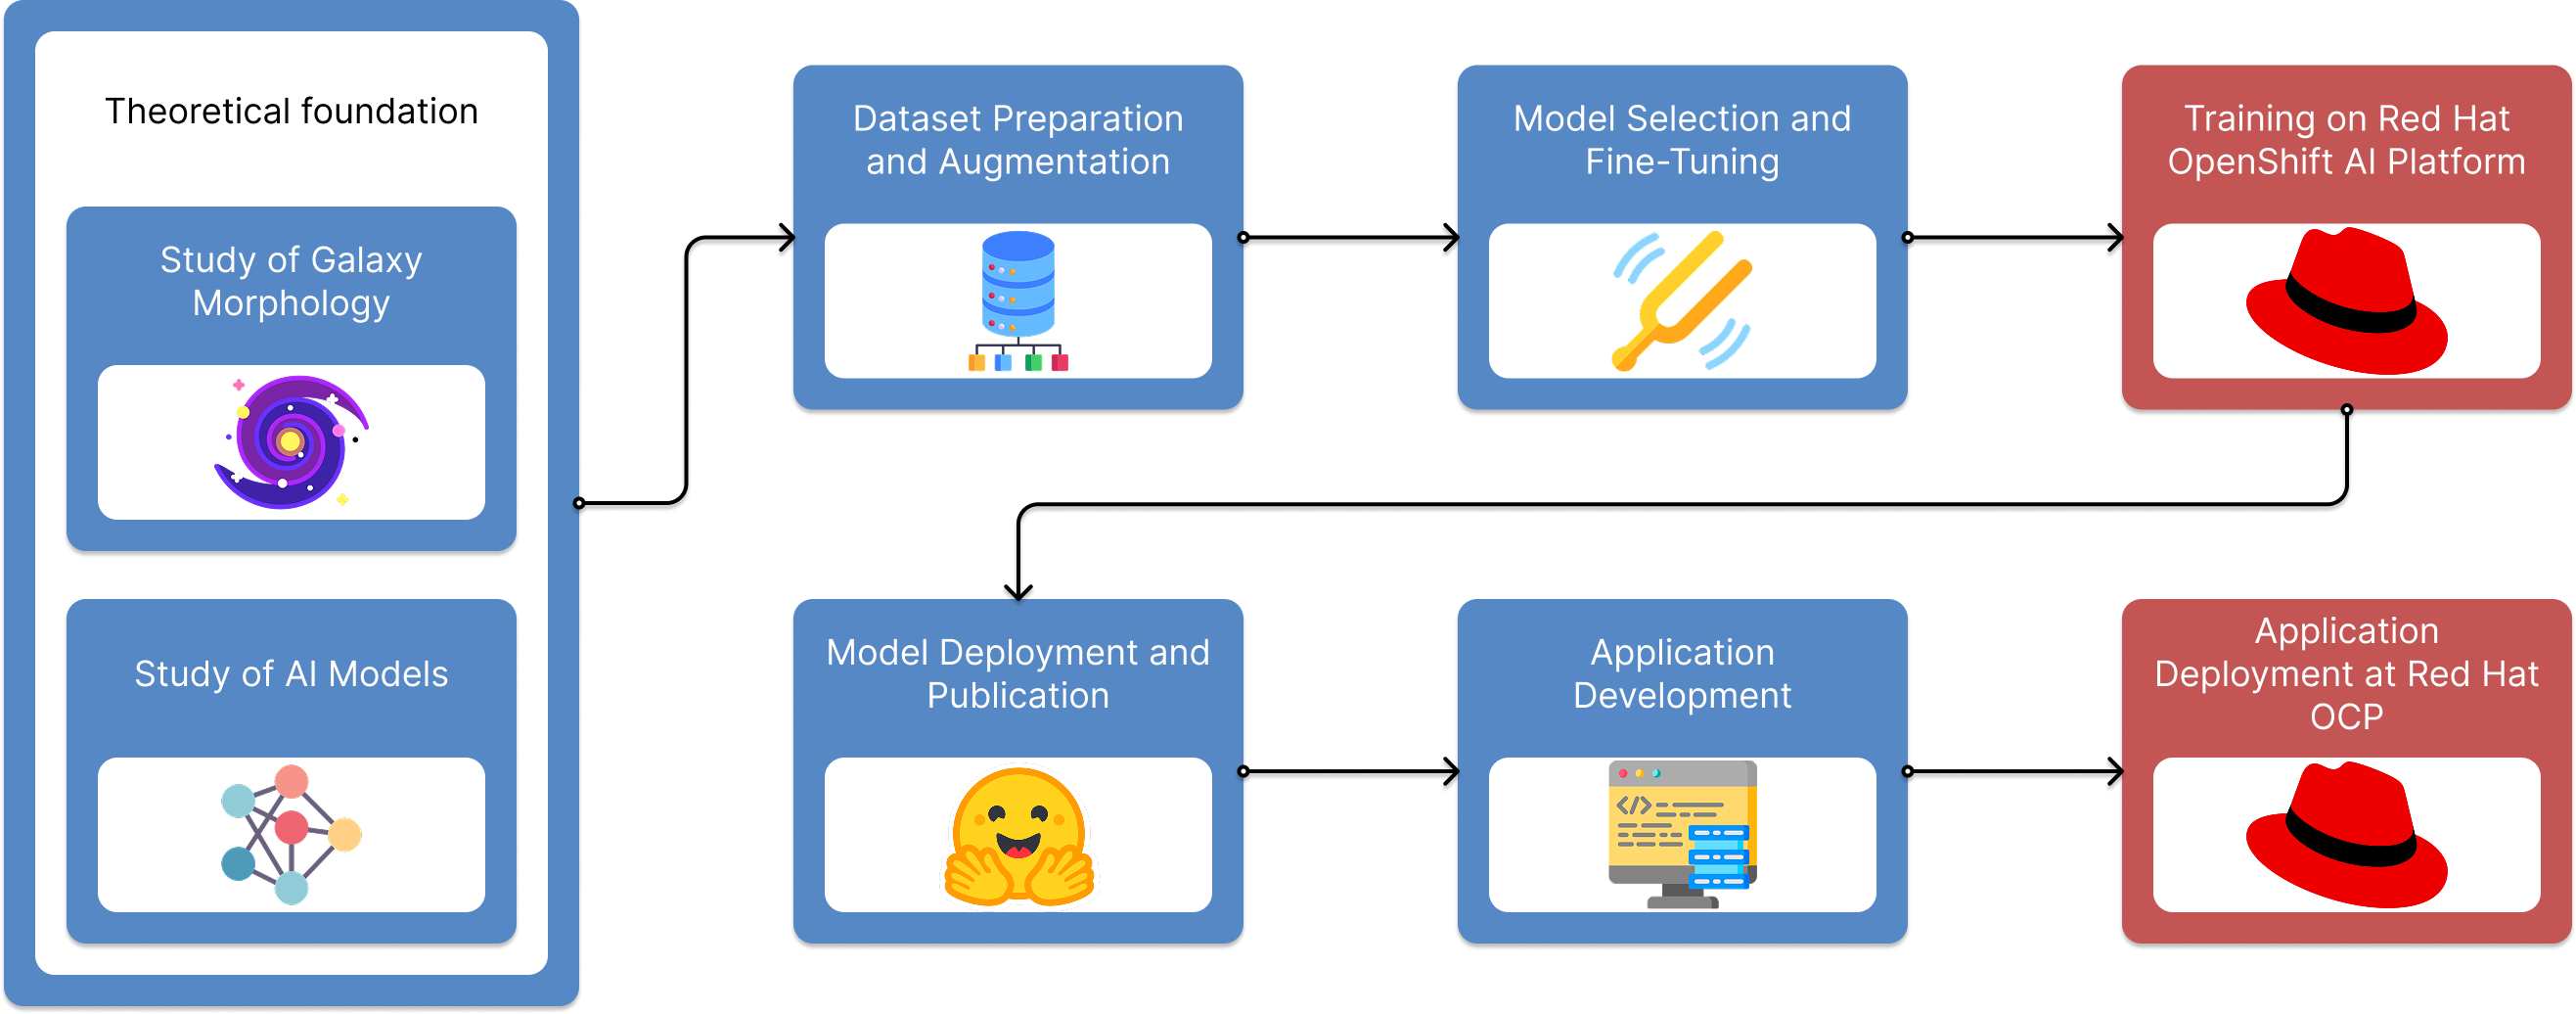
\includegraphics[width=\textwidth]{obrazky-figures/04-draft/pipeline.png}
  \caption{High-level implementation pipeline for the CosmoFormer application}
  \label{fig:pipeline}
\end{figure}

Each phase of web application development is viewed as straightforward and comprehensible. The objectives are well-defined and the outcomes are attainable. Bearing this development guide in mind, we can delve into the process of application implementation.

\chapter{Implementation}
\label{chapter:implementation}

This chapter documents the implementation of the final application, which involves transforming the application draft into working code, a trained model, containerized services, and Red Hat OpenShift deployment. We will start with processing and division of the Galaxy Zoo 2 dataset for training, validation, and testing subsets. Then we will focus on the defining of the CrossFormer model using \texttt{vit-pytorch} and PyTorch, along with strategies for optimizing the model for inference. Subsequently, model will be trained on the partitioned dataset. After achieving consistent results or reaching the training bound, the model will be saved as TorchScript and published on Hugging Face. We will continue with a FastAPI-based backend to load the trained model, process image uploads, and return morphology predictions through a REST endpoint. Concurrently, we will develop a React-based frontend using the NGINX web server, offering a straightforward upload interface and showing classification outcomes to users. Finally, we will describe the containerization of both the frontend and backend, set up CI/CD workflows for automated build images and push them into Quay.io. After that, we will declare yaml manifests with resources' definitions (Deployments, Services, Routes, HPAs, ResourceQuotas) for deployment and operation on the Red Hat OpenShift Container Platform\footnote{The complete source code is available at \url{https://github.com/ArturSultanov}}. Final model is called \enquote{CosmoFormer.} This name emphasizes that the model will be based on a CrossFormer architecture and will be trained on a galaxy dataset.

\section{Red Hat OpenShift AI setup}

In the previous section, we have organized the dataset into partitions for training, validation, and testing purposes. We now proceed to define the model using \texttt{vit-pytorch} and create a training loop with \texttt{PyTorch}. Training a model demands substantial computational resources, and a graphics accelerator typically speeds up the model’s training process. Nonetheless, contemporary AI-capable GPUs with a large amount of VRAM are quite expensive. To address this, Red Hat OpenShift AI, a cloud-based platform with GPUs dedicated for AI workloads, will be utilized to train the CosmoFormer model.

\subsection*{Workbench setup}

Red Hat OpenShift AI provides a Data Science Project to users, which encapsulates preconfigured notebook workbenches, secure data connectors, scalable storage, and integrated CI/CD pipelines.

\medskip

Before writing any code, we first need to set up a Workbench within our Data Science Project. The Workbench serves as a Jupyter notebook environment for developing and experimenting with machine learning. While setting up the Workbench, we can choose a notebook image. \enquote{PyTorch} image is used, because it is specially optimized for model development and comes with all the necessary tools and libraries already preinstalled.\footnote{Documentation is available at \url{https://docs.redhat.com/en/documentation/red_hat_openshift_ai_cloud_service/1/html/openshift_ai_tutorial_-_fraud_detection_example/creating-a-workbench-and-a-notebook\#creating-a-workbench}}. After configuring all properties, the Workbench will be started. Clicking 'Open' will redirect us to the Jupyter notebook environment, with GPU access and a configured persistent volume to store the data. 

\medskip

To verify whether our workbench is connected to the GPU, we should execute the \texttt{nvidia-smi} command in the terminal. As it is shown at \autoref{lst:gpu} \texttt{NVIDIA A10G} GPU is available for model training in the workbench environment. This GPU is equipped with \texttt{23,028 MiB} of VRAM, which should be sufficient for training model training such as CosmoFormer. Nevertheless, remember that for larger models, like LLMs with billions of parameters, a more advanced GPU might be needed.

\medskip

\begin{lstlisting}[style=mypython, caption={nvidia-smi command output}, label={lst:gpu}]
+------------------------------------------------------------------------+
| NVIDIA-SMI 570.124.06  Driver Version: 570.124.06     CUDA Version: 12.8     |
+------------------------------------------------------------------------+
| GPU  Name                Persistence-M | Bus-Id          Disp.A | Volatile Uncorr. ECC |
| Fan  Temp   Perf          Pwr:Usage/Cap |           Memory-Usage | GPU-Util  Compute M. |
|                                         |                        |               MIG M. |
|========================================================================|
|   0  NVIDIA A10G                    On  |   00000000:00:17.0 Off |                    0 |
|  0%   32C    P8             25W /  300W |       1MiB /  23028MiB |      0%      Default |
|                                         |                        |                  N/A |
+------------------------------------------------------------------------+
                                                                                         
+------------------------------------------------------------------------+
| Processes:                                                                              |
|  GPU   GI   CI              PID   Type   Process name                        GPU Memory |
|        ID   ID                                                               Usage      |
|========================================================================|
|  No running processes found                                                             |
+------------------------------------------------------------------------+
\end{lstlisting}

\section{Galaxy Dataset Preparation}
\label{sec:05-dataset}

This section will describe the process of dividing the original GZ2 dataset into training, validation, and test partitions. 

\subsection*{Dataset Loading and Partitioning}

Initially, we need to choose the development environment. While it's possible to write a basic Python script, it is preferred to use a Jupyter notebook. Because it brings an opportunity to display the output of each step, and this improves the clarity of the work. Consequently, following code will be designed to be executed within a Jupyter notebook.

First step, will be to define and install the Python packages which will be used during work with the dataset. As we discussed in \autoref{sec:draft-dataset} the core function for dataset partitioning is \texttt{scikit-learn}, \texttt{pandas} will be used for work with \texttt{DataFrames} type. We need to download dataset files, including labels and images. To do so we use \texttt{galaxy-datasets} Python package. Consequently, datasets are downloaded locally, allowing us to handle them using \texttt{pandas DataFrames}. If any labels are absent, they should be completed with the \enquote{Irregular} galaxy classification. Refer to \autoref{lst:data-load} for a code example\footnote{Final dataset, is available at \url{https://github.com/ArturSultanov/cosmoformer-dataset}}.

The training dataset comprises 167,434 samples, and the test dataset includes 41,859 samples. We can divide the training dataset to create a validation set. To achieve this, allocate 25\% of the training dataset using \texttt{sklearn.model\_selection.train\_test\_split} with a fixed random seed for reproducibility. Refer to  \autoref{lst:data-split} for the code example. Thus, the training subset size is 125,575 samples; the validation subset contains 41,859 samples; the test subset also contains 41,859 samples. Now we can save these three datasets as separate partitions in parquet format using \texttt{pandas.DataFrame.to\_parquet} method as shown in \autoref{lst:data-save}. After this, the following files and directories will be created:

\begin{itemize}
    \item \textbf{\texttt{test.parquet}:} Parquet file with test dataset labels.
    \item \textbf{test:/} Directory containing test dataset images.
    \item \textbf{\texttt{train.parquet}:} Parquet file with training dataset labels.
    \item \textbf{train/:} Directory containing training dataset images.
    \item \textbf{\texttt{validation.parquet}:} Parquet file with validation dataset labels.
    \item \textbf{validation/:} Directory containing validation dataset images.
\end{itemize}


\begin{figure}[htbp]\centering
  \centering
  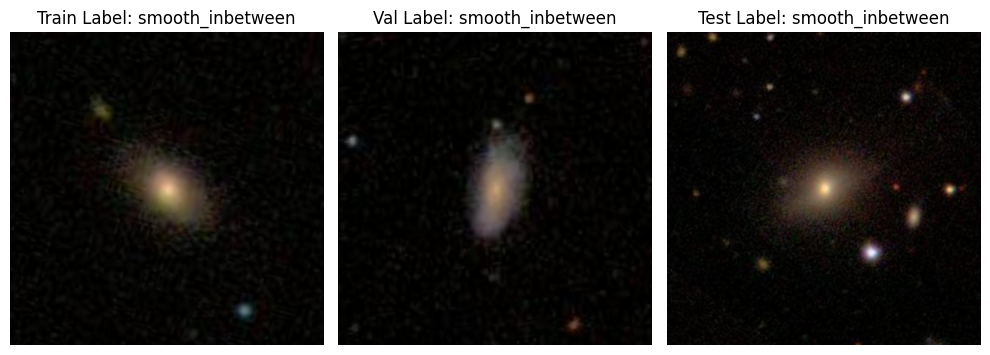
\includegraphics[width=\linewidth]{obrazky-figures/05-implementation/final-dataset.png}
  \caption{Examples of images from each of the three sub-sets after partitioning.}
  \label{fig:final-dataset}
\end{figure}

\subsection*{Data Augmentation}

During the training process, the model will utilize the re-partitioned dataset which has been defined and saved. Also, we would like to apply the augmentation described in \autoref{sec:03-data-augmentaiton}. Therefore, we need to create a \texttt{Dataset} and \texttt{DataLoader} \cite{siddiqui2025mastering}. 

In PyTorch, the \texttt{Dataset} class serves as an abstract representation of the used dataset, acting as a mapping from keys to data samples. \texttt{Dataset} subclass defined for our model reads the \texttt{Parquet} file, loads RGB images with \texttt{Pillow},  applies a transform pipeline and encodes text labels through a \texttt{scikit‑learn} label encoder. Refer to \autoref{lst:data-Dataset} for a code example.

\texttt{DataLoader} is a PyTorch class that allows handling data loading and processing in batches. When a \texttt{Dataset} is used with \texttt{DataLoader}, each sample of the dataset will be yielded from the \texttt{DataLoader} iterator. This means that we do not need to load all the data into memory at one time. The model can be trained on smaller batches of the dataset. DataLoader enhances the handling of large datasets by automatically managing shuffling, batching, and multiprocessing. It also allows the application of data augmentation (randomly) to each batch during training loops. The reference code example is shown at \autoref{lst:data-DataLoader}.

The last step to make our dataset ready-to-use is to define the augmentation, which has been described in \autoref{sec:03-data-augmentaiton}. You may want to use a predefined augmentation, which can be applied to the entire dataset prior to initiating the training process. For example, we can double the number of samples by incorporating augmented images into the original dataset. This method helps to increase the total number of samples in the dataset, which is particularly useful for smaller datasets. However, given that our training subset is relatively big and contains 125,575 samples, that pre-flight augmentation is unnecessary. Moreover, through experimentation with various augmentation techniques, it became clear that, in our scenario, pre-flight augmentation worsens performance by extending training time and causing model overfitting. Therefore, we will employ on-the-fly augmentation, when new augmentations are applied during each loop iteration to enhance the randomization effect of the augmentation.

For augmentation purposes, the PyTorch framework's \texttt{torchvision.transforms} will be utilized. This package offers several sophisticated augmentation methods. We establish two \texttt{torchvision.transforms.v2} pipelines. The training pipeline incorporates random resized cropping, flipping, color jitter, blurring, and rotation. Those techniques were described at \autoref{sec:03-data-augmentaiton}. While the validation pipeline employs a simple resize to align with the model input window. It is necessary to note that the image resizing to 224 by 224 pixels is dictated by the CrossFormer architecture. The CrossFormer implementation available through \texttt{vit-pytorch} accommodates an input window of 224 by 224 features. 

\section{CosmoFormer Model}

This section discusses aspects related to model optimization, training, and publication for further integration in the application. It also covers the results of the training and accuracy evaluation on the test subset.

\subsection*{Hyperparameters Optimization}
\label{sec:model-optimizations}

Training an AI model can be demanding on hardware resources. Since this thesis primarily emphasizes demonstrating the development and deploying processes instead of maximizing accuracy, the internal representation of the model will be reduced. This approach allows us to utilize fewer resources and reduce the duration required per training epoch.

In exploration of model hyperparameters, it has been discovered that reducing the model's \texttt{dim} (i.e., neurons per layer) is particularly beneficial. This adjustment not only decreases the model's size and training time but also maintains a similar level of accuracy. In contrast, modifying \texttt{depth} (number of layers) is vital for enhancing the learning potential, especially when working with a galaxy dataset. Consequently, the \texttt{dim} was halved: reduced from \texttt{(64, 128, 256, 512)} to (32, 64, 128, 256). Conversely, the \texttt{depth} parameter stayed at \texttt{(2, 2, 4, 2)}, by adjusting the third layer's block, which represents the coarsest intermediate resolution. Additionally, \texttt{attn\_dropout} and \texttt{ff\_dropout} both set to 0.1, which randomly zeroes out attention weights and feedforward activations during training. This acts as a regularizer, aiding in preventing overfitting, stabilizing convergence, and enhancing generalization for the galaxy dataset. The optimized definition of the model is provided in \autoref{lst:model-model}.

\begin{table}[hbt]
\centering
\caption{Comparison of Original and Optimized Models}
\label{tab:model_comparison}
\begin{tabular}{|l|c|c|c|}
\hline
Metric & Original & Optimized & Reduction \\ \hline
VRAM usage & 10 GiB & 6 GiB & 40\% \\ \hline
Epoch duration & 18 minutes & 8 minutes & 55\% \\ \hline
\end{tabular}
\end{table}

At \autoref{tab:model_comparison} we can see the comparison between the optimized and original versions. Overall, we can see an improvement in VRAM usage of about 40\% and  reduction in training time by about 55\%.\footnote{This comparison applies to training with half-precision or utilizing \texttt{autocast} and \texttt{GradScaler}.}

\subsection*{Training Process}

Now that we possess both the dataset and the model, we can start the training. We should create a training loop. To enhance the efficiency and stability of our model training process, we will utilize automatic mixed-precision (AMP). For this purpose, PyTorch provides \texttt{autocast} and \texttt{GradScaler}. In the training loop, we wrap our forward pass in an \texttt{autocast} block so that compatible operations run in 16-bit (FP16) instead of 32-bit (FP32). This approach significantly reduces GPU memory usage by half and accelerates calculations on modern CUDA-capable hardware. Given that FP16 can lead to the disappearance of very small gradients, we employ a \texttt{GradScaler} to adjust the loss before the backpropagation step. After computing gradients, the scaler “unscales” them so we can safely apply gradient clipping and update the optimizer, then adjusts its own scale factor up or down each step to catch any numerical overflow or underflow.

First of all, we need to select an appropriate learning rate. This hyperparameter dictates the effect level to which the model's weights are adjusted based on the estimated error at every update, thus balancing between fast convergence and stable training. To identify the best learning rate, we can employ the \textit{LRFinder}. Nonetheless, it is recommended to begin with a larger learning rate and then gradually reduce it. This can be managed using a \textit{Learning Rate Scheduler}. In setting up the scheduler, 10\% of the total epochs are allocated to a warm-up phase, during which the learning rate linearly escalates from zero to its base value. Following the warm-up, we transition to a cosine decay schedule: as the training advances, the learning rate decreases smoothly from the base down to zero. This is implemented by using the \texttt{LambdaLR} scheduler, which adjusts the optimizer’s base learning rate using our warm-up or cosine multiplier each epoch.

For optimizer, we employ \textit{AdamW}, an enhancement of Adam that separates weight decay from the gradient-based parameter updates. \textit{AdamW} preserves per-parameter learning rates by tracking the first (mean) and second (variance) moments of the gradients. This capability allows it to adjust the scale of individual updates while consistently applying a penalization to the weights at every step. By initializing this optimizer with an appropriate base learning rate and employing effective regularization, we achieve both rapid, noise-resistant convergence and improved generalization. The best model weights during the loop are being saved as checkpoints in \textit{.pth} format. As the result of the model is being trained on the GZ2 dataset and is capable of predicting the galaxy morphology class. To evaluate the final accuracy, the model is examined on the test sub-set, which has never been seen by the model. For code references see \autoref{lst:loop-setup}, \autoref{lst:loop-train}, \autoref{lst:loop-val}, \autoref{lst:loop-test}.

\subsection*{Model Accuracy Results}
\label{sec:model-results}

The final loss and accuracy of the Cosmoformer model on the test subset are following: \texttt{Test Loss: 0.8010} and \texttt{Test Acc: 0.7599}. Neither additional training nor enhancing the dataset increased the accuracy. Therefore, 75.99\% is considered as the accuracy borderline  for this model.

The authors of the research \enquote{Galaxy Morphological Classification with Efficient Vision Transformer} \cite{lin2022galaxymorphologicalclassificationefficient} share the accuracy metrics of various models on the test set\footnote{Available at: \url{https://github.com/soliao/Galaxy-Zoo-Classification/blob/main/vit_params.md}}. This allows us to evaluate our model's performance in comparison with their results.

\begin{table}[hbt]
\centering
\caption{Comparison with the CosmoFormer model}
\label{models-compare-trained}
\begin{tabular}{|l|c|c|}
\hline
Model Architecture & Trainable Parameters & Test Accuracy \\ \hline
Vision Transformer & 6,953,992	 & 81.17 \\ \hline
Vision Transformer (ArXiv params) & 3,663,240 & 79.57 \\ \hline
CrossFormer (CosmoFormer model) & 5,497,980 & 75.99 \\ \hline
\end{tabular}
\end{table}

In summary, our final model achieves a test accuracy of 75.99\% while utilizing slightly less than 5.5 million parameters. At \autoref{models-compare-trained}, we can see that our trained model exhibits competitive efficiency relative to the conventional ViT. Nevertheless, there is evident potential for further enhancements through refined tuning of learning rates, weight decay, warm-up schedules, or other hyperparameters.

\subsection*{Weights Saving and Publishing}

Since our model has been successfully trained on the dataset, we are ready to save and publish it. To enhance portability and minimize additional dependencies, we convert our trained model into a standalone \textit{TorchScript} artifact, enabling it to be loaded and executed on any backend without the necessity of the original Python script. Internally, \textit{TorchScript} make a snapshot of the model's control flow and parameters into a graph that can be statically analyzed. Then it stores the serialized model along with its weights in a single \textit{.pt} file. This makes deployment lightweight, portable across Python runtimes, and eliminates the requirement to integrate the full model code in a production environment. Reference code is listed at \autoref{lst:model-save}.

To make it publicly accessible, model is uploaded to the Hugging Face (HF). HF is a popular open-source platform where researchers and developers host and share machine learning models, datasets, and more. By hosting our model on HF, users can effortlessly download, experiment with, and integrate the model using a straightforward API or a repository. The repository \texttt{artursultanov/cosmoformer-model}\footnote{Available at \url{https://huggingface.co/artursultanov/cosmoformer-model}} provides the trained weights of the model, \textit{TorchScripts} files for both CPU and CUDA versions, as well as instructions for integrating the model.

\section{Backedn and Frontend}

The backend utilizes a REST API to interact with the frontend, using the FastAPI framework. FastAPI is a modern, high-performance, web framework for building APIs with Python based on standard Python type hints. It is responsible for loading the trained CosmoFormer model, handling inference requests, and providing the predicted galaxy classification. Although the purpose of the backend service is clear, there are several things to consider. Uvicorn was used as the web server. Uvicorn implements a multi-process model with one main process, which is responsible for managing a pool of worker processes and distributing incoming HTTP requests to them. As we discussed in \autoref{sec:draft-be}, the core functionality is implemented in the FastAPI Python framework, while \textit{uvicorn} serves as a web server. 

Due to \textit{FastAPI} documentation, we need to create an instance of \texttt{FastAPI} class to initialize the application. Also, using \texttt{@asynccontextmanager} decorator we define function \texttt{lifespan(app: FastAPI)}, which includes the code that should be executed before the application starts up. This means that this code will be executed once, before the application starts receiving requests. This is particularly useful to load our CosmoFormer model, which will be shared among requests, rather than loading one model per request.

Now we need to create a class that represents our model. Each instance of this class will load the \textit{TorchScript} artifact containing CosmoFormer. This class should have a method for handling the inference requests and returning the predicted galaxy class. In the web application, a CPU version of the model is used, because the deployment server could not have enough GPU resources. 

The next step involves incorporating the handler for user inference requests. Users will upload images that need processing by the model. \texttt{@app.post("/inference")} decorator tells the server to execute the corresponding function whenever a \textit{POST} request is sent to \texttt{https://cosmoformer:8000/inference}. 

Finally, we need to configure the \textit{Uvicorn} server to host our \textit{FastAPI} application as an \textit{ASGI} server, making the endpoints accessible externally. \textit{Uvicorn} is capable of managing requests asynchronously by leveraging CPU threads and specifying the worker count. Since various systems have different CPU configurations, \texttt{entrypoint.sh} script has been written. To detect the number of CPU threads, the script runs the following command: \texttt{exec uvicorn main:app --host 0.0.0.0 --port 8000 --workers "\$WEB\_CONCURRENCY"}. This helps dynamically identify the number of available CPU threads and prevents the need to hard-code the number of \textit{Uvicorn} workers. Executing this script initiates \textit{FastAPI} application at the address \texttt{0.0.0.0:8000}. For code references see \autoref{lst:be-life}, \autoref{lst:be-model}, \autoref{lst:be-post}.

JavaScript was selected for the frontend, which was explained in \autoref{sec:draft-fe}. Interactive elements are developed using the \texttt{React} library, with the UI designed as a single-page site. \textit{React-dropzone} is used to handle image uploads. It offers a simple React hook for creating an HTML5-compliant drag-and-drop area for files. The frontend sends POST requests to the backend API, processes the responses, and displays the predicted galaxy class to the user. An example of code is provided at \autoref{lst:fe-dz}. NGINX functions as a web server holding static content and acts as a reverse proxy, routing requests to the backend API.

\begin{figure}[htbp]
  \centering
  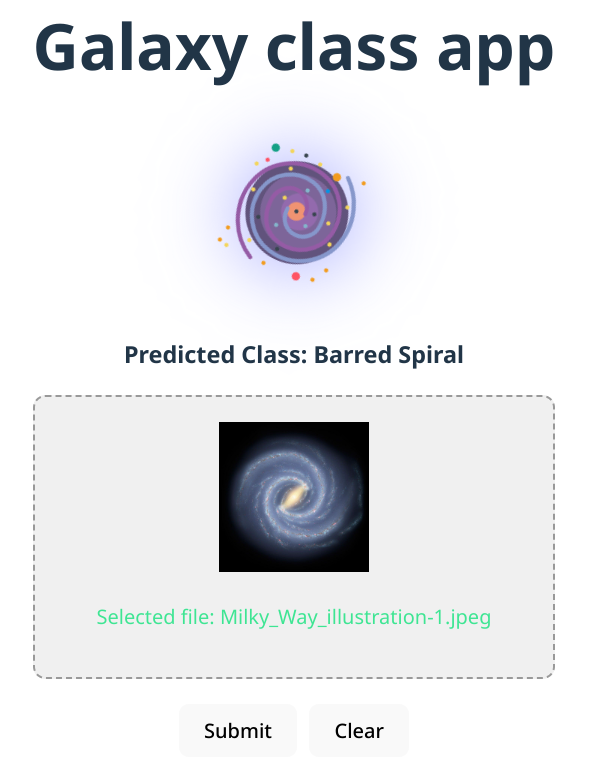
\includegraphics[width=0.5\textwidth]{obrazky-figures/05-implementation/ui.png}
  \caption{High-level implementation pipeline for the CosmoFormer application}
  \label{fig:ui}
\end{figure}

The completed design is shown in \autoref{fig:ui}. Below, there is a drop zone designated for image preview and upload. There are two buttons, “Submit” and “Clear,” which are used to process the request and delete the uploaded image, respectively.

\section{Openshift Deployment}

To deploy the application on the OpenShift cluster, it is necessary to containerize both the backend and frontend. This process involves creating Docker images and uploading them to a public registry. The backend image uses \texttt{quay.io/fedora/python-312-minimal} as its base and is enhanced with the \texttt{torchvision} and \texttt{torchv} packages to handle the CosmoFormer model. For the frontend, \texttt{quay.io/fedora/nodejs-22-minimal} serves as the builder image to generate static web application files. The base image of choice is \texttt{quay.io/nginx/nginx-unprivileged}, which runs NGINX as a non-root, unprivileged user. The selection of \texttt{nginx-unprivileged} aligns with OpenShift’s Security Context Constraints, which often restrict containers that require root access, especially in shared environments.

Because Openshift is designed to create pods by pulling images. Therefore, we need to publish images into the public image registry such as `quay.io`. So images will be accessible for our deployments.

After pushing images, application deployment into Red Hat OCP can proceed. The first step involves specifying the scope for OpenShift resources. To establish backend and frontend containers, we utilize a \texttt{Deployment}, which automatically generates \texttt{ReplicaSet}s  for these containers, sets memory and CPU limits, and handles labels and metadata for all underlying resources. Containers in the OpenShift run inside the \texttt{Pods}. To make the backend and frontend pods accessible within the cluster's software-defined network (SDN), a \texttt{Service} is necessary. The \texttt{Service} specifies the port that communicates with the container inside the pod. However, to make the frontend accessible from outside the cluster network, a \texttt{Route} resource is required. This creates an external hostname and TLS termination to route incoming HTTP traffic from outside the SDN directly to the frontend's entry-point port.

To enhance the robustness and reliability of our application under heavy load, it is essential to implement autoscaling features. For this, we employ \texttt{Horizontal Pod Autoscaling}, which dynamically adjusts pod capacity during increased traffic. HPAs keep the number of pod replicas in the range from 1 to 5 for each service. For both backend and frontend, the memory threshold is set at \texttt{averageValue: 3840Mi} and CPU utilization at \texttt{averageUtilization: 70}. It leverages liveness and readiness probes to identify and replace malfunctioning containers automatically, ensuring smooth recovery from pod failures or stalls.

\label{resquota}
The last \enquote{cherry on top} is using resource management to prevent our application from overconsuming resources, which could disrupt other tasks within the same namespace or even affect the entire cluster. This can be achieved by implementing \texttt{ResourceQuota}. This dictates the maximum number of pods that can exist simultaneously, the amount of CPU and memory allocated for the entire project, and the specific resource limits. The \texttt{limits.cpu: "10"} and \texttt{limits.memory: "32Gi"} were applied to limit the resource usage.

The final set of needed resources is listed below: 

\begin{itemize}
  \item \textbf{Deployments}
    \begin{itemize}
      \item \texttt{cosmoformer-backend-deployment}: defines the Pod template for the FastAPI backend image.
      \item \texttt{cosmoformer-frontend-deployment}: defines the Pod template for the React frontend image.
    \end{itemize}
    
  \item \textbf{Services}
    \begin{itemize}
      \item \texttt{cosmoformer-backend-service}: exposes the FastAPI Pods internally (ClusterIP) for in-cluster communication.
      \item \texttt{cosmoformer-frontend-service}: exposes the React Pods internally so the Route can direct external traffic.
    \end{itemize}

  \item \textbf{Route}
    \begin{itemize}
      \item \texttt{cosmoformer-frontend-route}: maps an external hostname to the frontend Service, handling TLS and load-balancing. Frontend calls under \texttt{/api/} are proxied to the backend Service.
    \end{itemize}

  \item \textbf{ResourceQuota}
    \begin{itemize}
      \item \texttt{cosmoformer-rq}: enforces CPU, memory, and pods limits within the project to prevent resource over-consumption on the shared cluster.
    \end{itemize}

  \item \textbf{HorizontalPodAutoscalers}
    \begin{itemize}
      \item \texttt{cosmoformer-backend-hpa}: monitors metrics and scales the backend between defined min/max replicas.
      \item \texttt{cosmoformer-frontend-hpa}: similarly scales the frontend based on load.
    \end{itemize}
\end{itemize}

The \texttt{kustomize} utility is employed to create resource manifests and subsequently merge them into a consolidated manifest. Additionally, \texttt{kustomize} verifies that the complete manifest is free of syntax errors prior to its application to the cluster. 

With the manifest of all deployment resources completed, we are ready to deploy our application on Openshift. We will use a hybrid-cloud Red Hat OCP solution. Though, \textit{CodeReady Containers (crc)} is suitable for local testing and experiments\footnote{Further details about crc can be found at \url{https://developers.redhat.com/products/openshift-local/overview}}.

In order to access the target deployment cluster, it is necessary to install the \textit{oc} CLI tool. This tool allows for management of the cluster through the OpenShift console API. Once logged into the cluster with \textit{oc}, a \texttt{Project} can be created to encapsulate all application's components into one namespace. Then we can apply the deployment manifest using the command \texttt{oc apply -f manifest.yaml}. In order to streamline the deployment process and minimize the possible mistakes, it is recommended to use a script that automates the construction and application of the manifest.

\section{Tests and Performance}
\label{sec:testing}

Testing is crucial for identifying errors, vulnerabilities, and weaknesses in applications. To keep implementation steps clear, all testing methods and tools are consolidated into this section.

\subsection*{API tests}

Tests, which cover all API methods, are implemented with \textit{pytest}. This framework allows developers to write simple tests in \textit{Python} language. It is easy and straightforward to use for test creation. The main feature is that the framework tracks the tests that should be executed based on the functions' names. Therefore, test functions should start with \texttt{test\_} prefix. The purpose of  each test function is listed below.

\begin{itemize}
  \item \texttt{test\_root()}: verifies if the root URL \texttt{https://cosmoformer:8000/} is accessible.
  \item \texttt{test\_healthcheck()}: evaluates the \texttt{/healthcheck} endpoint to ensure that the application has started.
  \item \texttt{test\_readycheck()}: evaluates the \texttt{/readycheck} endpoint to ensure that the \textit{CosmoFormer} model is initialized and ready.
  \item \texttt{test\_inference\_for\_all\_images()}: sends images to \texttt{/inference} endpoint using the \textit{POST} method to verify the availability of the \textit{CosmoFormer} model for performing inference.  
\end{itemize}

\subsection*{Kustomize tests}

Test scripts utilizing the \textit{kustomize} tool are employed to verify the accurate declaration of our OpenShift manifests.

\begin{itemize}
  \item \texttt{test\_kustomize\_build.sh}: builds the overlay with \texttt{kustomize build} and writes the rendered manifest to \texttt{/tmp/cosmoformer\_openshift.yaml}. It also prints a summary of generated resource and the full \textit{YAML} to \textit{stdout}.
  \item \texttt{test\_kustomize\_dry\_run.sh}: takes the rendered manifest and runs command \texttt{oc apply --dry-run=client} to ensure the YAML is syntactically valid for the OpenShift API. It exits with an error if the manifest is missing or the dry‑run fails.
\end{itemize}

\subsection*{Performance test}

The performance test uses the k6 framework to test and measure the throughput and latency of the \texttt{/inference} endpoint. It simulates the scenario when users constantly upload images via the application endpoint. This also allows checking if \texttt{HorizontalPodAutoscaler}s  work as expected. 

The script executes a “ramping‑vus” scenario of performance and stress tests. This scenario starts with increasing the  virtual users (VUs) from 0 to 5 in the first 10 seconds, keeps 5 users active for 280 seconds, then ramps back down to 0 during the final 10 seconds.The delay between requests of one user is 5 seconds, which simulates the time needed for a real person to upload an image. The entire testing time is 5 minutes. 


\begin{table}[hbtp]
\centering
\caption{Performant test results}
\label{tab:ptest}
\begin{tabular}{|l|c|c|c|}
\hline
Metric          & Total & Succeeded & Failed    \\ \hline
Number requests & 184   & 118       & 66        \\ \hline
Percentage      &       & 64.13\%   & 35.86\%   \\ \hline
\end{tabular}
\end{table}

The outcomes of this test are presented in \autoref{tab:ptest}. It is observed that merely 64.13\% of all requests in the performance test were successful. While the desired performance goal was not met, the results indicate that the application is functioning correctly. To determine the root cause of the issue, we should examine the project's metrics.

\begin{figure}[htbp]\centering
    \centering
    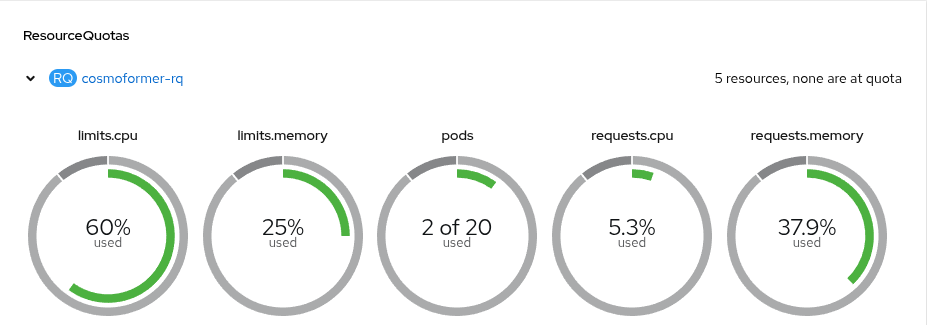
\includegraphics[width=0.8\linewidth]{obrazky-figures/05-implementation/no-load.png}
    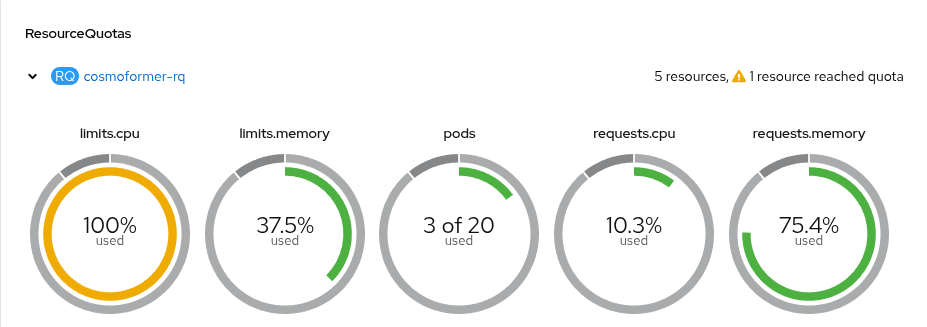
\includegraphics[width=0.8\linewidth]{obrazky-figures/05-implementation/load.png}
    \caption{Comparison application without load (above) and under the load (below).}
    \label{fig:test-load}
\end{figure}

Based on the OpenShift metric depicted in \autoref{fig:test-load}, the primary factor causing the application to fail the test is a CPU bottleneck. As discussed in \autoref{resquota}, the application resource capacity is restricted by \texttt{ResourceQuota}, which sets the usage at \texttt{limits.cpu: "10"} and \texttt{limits.memory: "32Gi"}. Consequently, when the backend pods auto-scale, the project hits the CPU limit. This observation lets us highlight that the performance shortfall stems from project resource availability issues rather than the application design itself.

\section*{Final Application}

Following the preceding steps, our web application now successfully operates in the OpenShift environment. The deployment combines essential components into a production-ready system: a Deep Learning model that is trained and serialized, an API backend, and an intuitive frontend. When the website is accessed, NGINX serves the static assets produced by React. If an image is placed in the \enquote{drag-and-drop} area or chosen, the frontend sends the file to the backend API via a \texttt{POST} request. Within the backend, the CosmoFormer model executes inference, determines the predicted class, translates it into a galaxy type label, and sends it back as a JSON payload. The frontend then updates and shows the user the predicted galaxy type. From a platform perspective, the backend and frontend containers are running in separate pods, which are orchestrated by respective Deployments. Horizontal Pod Autoscalers monitor CPU and memory metrics and check pods' health and readiness. If usage exceeds set limits, additional replicas are spun up automatically, and requests are redistributed without any downtime. Combining all aspects together, the final application meets the initial requirements. This architecture results in a highly resilient and dynamically scalable cloud-native application that can be run in on-premises and public cloud OpenShift environments\footnote{The application source code is available at \url{https://github.com/ArturSultanov/cosmoformer-application}}.

\chapter{Discussion of the obtained results}

In this chapter, we analyze the results obtained and evaluate their implications.

The CosmoFormer model, based on a CrossFormer architecture, with approximately 5.5 million parameters, achieved a classification accuracy of 75.99\% on the Galaxy Zoo 2 test subset. This level of performance, when compared to the full-scale Vision Transformer which has 6.9 million parameters and achieves an accuracy of 81.17\%, shows that it has competitive efficiency considering its reduced parameter count and, accordingly, smaller resource demands.The reduction of the model’s hidden dimensions (from (64, 128, 256, 512) to (32, 64, 128, 256)) yielded a 40\% decrease in GPU memory usage (from 10 GiB to 6 GiB) and a 55\% reduction in per-epoch training time (from 18 minutes to 8 minutes). By reducing the dimensionality by half, this optimization highlights the balance between the model’s capacity and resource limitations, enabling the network to maintain consistent representational capability for galaxy morphology tasks while operating on less sophisticated hardware. Despite these gains, the observed 75.99\% accuracy suggests room for improvement. Potential factors limiting performance include class imbalance across galaxy types, the finite size of the Galaxy Zoo 2 subset, and the simplicity of the on-the-fly augmentation pipeline. Future work could explore more advanced augmentation strategies (e.g., elastic deformations, noise injections), class-aware sampling, or curriculum learning to better expose the model to rare morphologies. Additionally, experimenting with other hierarchical ViT variants (such as Swin or CvT) or ensembling multiple architectures may help close the gap to state-of-the-art accuracy.

From an application standpoint, the final web service meets the core functional requirements: users can upload arbitrary galaxy images via a React frontend, receive morphology predictions in real time, and benefit from automatic backend scaling on Red Hat OpenShift. The model has been serialized into a TorchScript artifact and served using FastAPI. The application features an intuitive UI and allows classifying galaxies' images. However, during the stress test, only 64.13\% of inference requests were completed successfully before encountering errors. An analysis of metrics showed that Horizontal Pod Autoscalers spun up additional replicas until the project's CPU quota was reached, causing request failures instead of application errors. This CPU bottleneck indicates that to achieve real-world scalability, one might need to either expand the cluster's CPU limits, transition inference to GPU-powered pods, or enhance request processing by employing batching and asynchronous pipelines. Additionally, implementing a caching layer for repeated inferences and using a more efficient model serialization method could potentially decrease latency and resource usage per request.

In summary, the CosmoFormer model and web-application validate that a lightweight ViT variant can perform galaxy morphology classification with reasonable accuracy while fitting within constrained compute budgets. The accompanying OpenShift deployment illustrates how to integrate AI workloads into a cloud-native environment with self-healing, autoscaling, and seamless frontend-backend integration. The results highlight both the promise of Transformer-based vision models in astronomy and the practical challenges of serving them at cloud platforms.


\chapter{Conclusion}
This thesis has explored the integration of contemporary computer-vision architectures for image classification into cloud-native infrastructure, with a focus on galaxy morphology analysis. CosmoFormer, a lightweight Transformer-based model, was created to operate within a computationally constrained environment and demonstrated its deployment within a Red Hat OpenShift Container Platform.

For robust feature extraction from galaxy images, we prepared and preprocessed the Galaxy Zoo 2 dataset, applying an advanced augmentation strategy to address class imbalance and improve generalization. The CosmoFormer model achieved accuracy comparable to existing models despite its reduced parameter count.

Building upon the trained model, we implemented a responsive full-stack web application. A RESTful backend initializes CosmoFormer at startup, while the frontend presents an intuitive interface allowing astronomers to upload images and receive real-time classifications. Containerized as Kubernetes pods on OpenShift, each component leverages horizontal autoscaling, health probes, and resource quotas to guarantee sub-200 ms response times under variable load and to maintain high availability.

Throughout the project, practical challenges in model training, resource provisioning, and continuous delivery were identified and addressed. This work highlights the advantages of containerization, cloud infrastructure, and dynamic resource management for sustaining modern AI workloads. The resulting deployment pipeline not only verifies the technical feasibility of hybrid-cloud AI systems but also establishes a reproducible blueprint for similar applications.

Looking forward, several directions may enhance and extend this research. On the AI model side, experimenting with hierarchical Transformer architectures could further improve classification accuracy, while refining the augmentation pipeline may mitigate residual class imbalances. From a systems perspective, integrating on-demand GPU inference or asynchronous processing would reduce latency during peak loads.

In conclusion, this thesis provides a solid foundation for the development of applications powered by AI. By combining advanced vision-transformer techniques with robust cloud-native deployment strategies, it offers a scalable solution to accelerate and make galaxy morphology studies more accessible to a wider audience.

%=========================================================================

% For compilation piecewise (see projekt.tex), it is necessary to uncomment it
% \end{document}